% ======================================================================
%  FYS4480/FYS9480  Quantum mechanics for many-particle systems
%  Week 47, November 19-20, 2026
%  Lecture slides (Beamer).  Thursday: 2 x 45 min,  Friday: 2 x 45 min.
%
%  Coupled-cluster doubles, step by step (chapter 10, sections 10.1-10.6,
%  10.9 and the CCD part of 10.14).
%  Thursday: the Friday lectures of week 46 (November 13) once more -- the
%  exponential ansatz, the similarity-transformed Hamiltonian, the finite
%  BCH expansion -- and then the CCD amplitude equation derived term by
%  term with Wick's theorem.
%  Friday: the same ten terms derived with diagrams, and CCD for the
%  pairing model in code (classes PairingModel, CCD, PairCCD of week47.ipynb).
%  No exercises this week (second midterm, deadline November 23).
%  Short answers to the week-46 exercises are on the last frames.
%  Companion notebook: week47.ipynb (numpy only).
%  Diagram styles (pline, hline, vint, vtx, fvtx, amp, fcidiagram) are those
%  of book.tex; the diagrams are those of chapter 10, generated by
%  BookPrograms/chapter10/ccsd_diagrams.py and embedded here.
%  Build: pdflatex week47.tex (twice).  No external figures needed.
% ======================================================================
\documentclass[aspectratio=169,10pt]{beamer}

% ---------------------------------------------------------------- packages
\usepackage[utf8]{inputenc}
\usepackage[T1]{fontenc}
\usepackage{lmodern}
\usepackage{amsmath,amssymb,bm,mathtools}
\usepackage{booktabs}
\usepackage[most]{tcolorbox}
\usepackage{listings}
\usepackage{hyperref}
\usepackage{tikz}
\usepackage{pgfplots}\pgfplotsset{compat=1.18}
\usetikzlibrary{positioning,arrows.meta,decorations.markings,shapes.misc}
\usetikzlibrary{tikzmark}

% ---------------------------------------------------------------- look
\usetheme{default}
\useinnertheme{rectangles}
\setbeamertemplate{navigation symbols}{}
\definecolor{uioblue}{RGB}{18,52,86}
\definecolor{teal}{RGB}{0,128,128}
\definecolor{warm}{RGB}{181,73,36}
\definecolor{paleblue}{RGB}{232,240,248}
\definecolor{paleteal}{RGB}{228,244,244}
\definecolor{palewarm}{RGB}{252,238,230}
\definecolor{palegreen}{RGB}{232,244,234}
\setbeamercolor{structure}{fg=uioblue}
\setbeamercolor{title}{fg=uioblue}
\setbeamercolor{frametitle}{fg=uioblue,bg=white}
\setbeamercolor{section in toc}{fg=uioblue}
\setbeamercolor{alerted text}{fg=warm}
\setbeamercolor{block title}{fg=white,bg=uioblue}
\setbeamercolor{block body}{bg=paleblue}
\setbeamercolor{block title example}{fg=white,bg=teal}
\setbeamercolor{block body example}{bg=paleteal}
\setbeamerfont{frametitle}{size=\large,series=\bfseries}
\setbeamerfont{title}{size=\LARGE,series=\bfseries}
\setbeamertemplate{frametitle}{%
  \vspace*{0.6em}\insertframetitle\par
  \vspace*{-0.2em}{\color{teal}\rule{\textwidth}{0.6pt}}}
\setbeamertemplate{footline}{%
  \hbox{\begin{beamercolorbox}[wd=\paperwidth,ht=2.4ex,dp=1.2ex,leftskip=1em,rightskip=1em]{structure}%
  \footnotesize FYS4480/9480 -- Week 47 \hfill \insertsectionhead \hfill \insertframenumber/\inserttotalframenumber
  \end{beamercolorbox}}}
\setbeamertemplate{itemize items}[circle]
\setbeamertemplate{enumerate items}[default]
\setbeamertemplate{section page}{%
  \begin{centering}
    {\usebeamerfont{section title}\usebeamercolor[fg]{title}\LARGE\bfseries\insertsection\par}
    \vspace{0.5em}{\color{teal}\rule{0.5\textwidth}{1pt}}
  \end{centering}}
\AtBeginSection[]{\frame{\sectionpage}}

% ---------------------------------------------------------------- boxes
\newcounter{thinkctr}
\newcommand{\thinkq}[2]{%
  \stepcounter{thinkctr}%
  \vfill
  \begin{tcolorbox}[enhanced,colback=palewarm,colframe=warm,boxrule=1.2pt,arc=4pt,
    grow to left by=6mm,grow to right by=6mm,
    left=16pt,right=16pt,top=16pt,bottom=18pt,
    fonttitle=\bfseries\Large,fontupper=\Large,
    title={Pause to think \#\thethinkctr\hfill\mdseries\normalsize(about #1 min -- discuss with your neighbour)}]
  #2
  \end{tcolorbox}
  \vfill}
\newcommand{\thinka}[1]{%
  \vfill
  \begin{tcolorbox}[enhanced,colback=paleteal,colframe=teal,boxrule=1.2pt,arc=4pt,
    grow to left by=6mm,grow to right by=6mm,
    left=16pt,right=16pt,top=16pt,bottom=18pt,
    fonttitle=\bfseries\Large,fontupper=\large,
    title={Answer to pause \#\thethinkctr}]
  #1
  \end{tcolorbox}
  \vfill}
\newcommand{\mbbox}[1]{%
  \begin{tcolorbox}[colback=paleblue,colframe=uioblue,title={\bfseries Many-body connection}]
  #1
  \end{tcolorbox}}
\newcommand{\warnbox}[1]{%
  \begin{tcolorbox}[colback=palewarm,colframe=warm,title={\bfseries A trap to avoid}]
  #1
  \end{tcolorbox}}
\newcommand{\numbox}[1]{%
  \begin{tcolorbox}[colback=palegreen,colframe=teal!70!black,title={\bfseries Measured}]
  #1
  \end{tcolorbox}}

% ---------------------------------------------------------------- code
\lstset{language=Python,basicstyle=\ttfamily\scriptsize,
  keywordstyle=\color{uioblue}\bfseries,commentstyle=\color{teal},
  stringstyle=\color{warm},showstringspaces=false,columns=fullflexible,
  frame=single,rulecolor=\color{paleblue},backgroundcolor=\color{white},
  breaklines=true}

% ---------------------------------------------------------------- macros
\newcommand{\ket}[1]{\vert #1\rangle}
\newcommand{\bra}[1]{\langle #1\vert}
\newcommand{\braket}[2]{\langle #1\vert #2\rangle}
\newcommand{\element}[3]{\langle #1\vert #2\vert #3\rangle}
\DeclareMathOperator{\tr}{tr}
\newcommand{\bigO}{\mathcal{O}}
\newcommand{\bmat}[1]{\bm{#1}}
\newcommand{\Amat}[1]{\bm{A}^{#1}}
\newcommand{\Bmat}[1]{\bm{B}^{#1}}
\newcommand{\hH}{\hat{H}}
\newcommand{\ad}[1]{a_{#1}^{\dagger}}
\newcommand{\ketbra}[2]{\vert #1\rangle\langle #2\vert}
% normal ordering with respect to the reference determinant |c> (as in week 40)
\newcommand{\nc}[1]{\bigl\{#1\bigr\}}

% ---------------------------------------------------------------- diagrams
\tikzset{
  tens/.style={draw=uioblue,fill=paleblue,thick,rounded corners=1pt,minimum size=7mm,font=\small},
  mpo/.style={draw=warm,fill=palewarm,thick,rounded corners=1pt,minimum size=7mm,font=\small},
  env/.style={draw=teal!70!black,fill=paleteal,thick,rounded corners=1pt,
              minimum width=7mm,minimum height=14mm,font=\small},
  leg/.style={thick,uioblue},
  dlab/.style={font=\scriptsize},
  every picture/.style={scale=0.8,baseline=(current bounding box.center)}
}



\newcommand{\dd}{\mathrm{d}}


% ---------------------------------------------------------------- MBPT macros
\newcommand{\mel}[3]{\langle #1\lvert #2\rvert #3\rangle}
\newcommand{\av}[1]{\langle #1\rangle_0}
\newcommand{\cre}[1]{a_{#1}^{\dagger}}
\newcommand{\ann}[1]{a_{#1}}
\newcommand{\no}[1]{\bigl\{#1\bigr\}}
\newcommand{\vbar}[4]{\overline v_{#1#2#3#4}}
\newcommand{\Eref}{E_{\mathrm{ref}}}
\newcommand{\ph}{\Phi_0}
\newcommand{\Psizero}{\Psi_0}
\newcommand{\ord}[1]{\mathcal O(#1)}
\newcommand{\Rzero}{R_0}
\tikzset{fermion/.style={line width=.8pt,uioblue,postaction={decorate},decoration={markings,mark=at position .56 with {\arrow{Stealth}}}},
  interaction/.style={dashed,line width=.8pt,warm},
  vertex/.style={circle,fill=warm,inner sep=1.7pt}}
% ---- the Goldstone-diagram styles of book.tex (chapter 5, 9 figures)
\tikzset{
  pline/.style={thick,uioblue,postaction={decorate},
    decoration={markings,mark=at position 0.55 with {\arrow{Stealth[length=5pt]}}}},
  hline/.style={thick,uioblue,postaction={decorate},
    decoration={markings,mark=at position 0.55 with {\arrowreversed{Stealth[length=5pt]}}}},
  vint/.style={dashed,thick,warm},
  vtx/.style={circle,fill=warm,inner sep=1.4pt},
  fvtx/.style={cross out,draw=warm,thick,minimum size=5pt,inner sep=0pt},
  dlab/.style={font=\scriptsize},
  hloop/.style={thick,uioblue,postaction={decorate},
    decoration={markings,mark=at position 0.5 with {\arrow{Stealth[length=5pt]}}}},
  fcidiagram/.style={scale=0.9,baseline=(current bounding box.center)}}
\newcommand{\ftil}[1]{\tilde f_{#1}}
\tikzset{amp/.style={line width=2.4pt,uioblue}}
\newcommand{\Hbar}{\overline{H}}
\newcommand{\as}[4]{\langle #1#2\Vert #3#4\rangle}
\newcommand{\W}{W}
\newcommand{\wickpattern}[1]{%
\begin{tikzpicture}[x=.86cm,y=.72cm,every node/.style={font=\small,inner sep=1.3pt},scale=1,baseline=(current bounding box.center)]
\node(p)at(0,0){\(\cre{p}\)};\node(q)at(1,0){\(\cre{q}\)};
\node(s)at(2,0){\(\ann{s}\)};\node(r)at(3,0){\(\ann{r}\)};
\node(a)at(4,0){\(\cre{a}\)};\node(b)at(5,0){\(\cre{b}\)};
\node(j)at(6,0){\(\ann{j}\)};\node(i)at(7,0){\(\ann{i}\)};
\draw[uioblue,line width=.6pt,rounded corners=3pt](p.north)--++(0,1.05)-|(i.north);
\draw[uioblue,line width=.6pt,rounded corners=3pt](q.north)--++(0,.64)-|(j.north);
\ifnum#1=1\relax
\draw[teal,line width=.7pt,rounded corners=3pt](s.south)--++(0,-.9)-|(b.south);
\draw[teal,line width=.7pt,rounded corners=3pt](r.south)--++(0,-.48)-|(a.south);
\else
\draw[teal,line width=.7pt,rounded corners=3pt](s.south)--++(0,-.9)-|(a.south);
\draw[teal,line width=.7pt,rounded corners=3pt](r.south)--++(0,-.48)-|(b.south);
\fi
\end{tikzpicture}}



% ---------------------------------------------------------------- week 47 additions
\lstdefinestyle{big}{basicstyle=\ttfamily\footnotesize,keepspaces=true}
\lstdefinestyle{mid}{basicstyle=\ttfamily\scriptsize,keepspaces=true}
\newcommand{\stepbox}[2]{%
  \begin{tcolorbox}[colback=paleblue,colframe=uioblue,title={\bfseries #1},left=4pt,right=4pt,top=2pt,bottom=2pt]
  #2
  \end{tcolorbox}}

% ---------------------------------------------------------------- title
\title{Coupled-cluster doubles, step by step}
\subtitle{FYS4480/FYS9480 -- Week 47, November 19--20, 2026}
\author{Cecilie Glittum and Morten Hjorth-Jensen}
\institute{Department of Physics,\\
University of Oslo, Norway}
\date{}


\begin{document}

\begin{frame}[plain]
  \vspace*{-0.7em}{\setbeamerfont{title}{size=\Large,series=\bfseries}\titlepage}
  \vfill
  \begin{center}\small
  Thursday: coupled-cluster theory once more -- the exponential ansatz and the similarity-transformed Hamiltonian -- and the CCD equation derived term by term with Wick's theorem\\
  Friday: the same equation derived with diagrams, and coupled-cluster doubles for the pairing model in code\\[0.55em]
  {\footnotesize Reading: lecture notes chapter 10, sections 10.1--10.6 (ansatz to the CCD equations), 10.9 (the pairing model) and the CCD diagrams of section 10.14. Shavitt and Bartlett, chapter 9, sections 9.1--9.4 and chapter 10, sections 10.1--10.4. Code: \texttt{BookPrograms/chapter10/coupledcluster.py}, \texttt{ccsd\_diagrams.py}; notebook \texttt{week47.ipynb}.\\[0.2em]
  No exercises this week: the second midterm is due November 23. Short answers to the week-46 exercises: last frames.}
  \end{center}
\end{frame}

\begin{frame}[shrink=3]{Plan for week 47}
\small
\begin{block}{Thursday: from the ansatz to the CCD equation, analytically}
\begin{itemize}
\item Lecture 1 (repetition of November 13): why $e^{T}$, the cluster operator, the similarity-transformed Hamiltonian, why the Baker-Campbell-Hausdorff series stops, the projected equations, and what CCD keeps.
\item Lecture 2: the CCD amplitude equation derived with Wick's theorem, one term at a time: energy, driving term, the two Fock terms, the two ladders, the ring, and the four quadratic terms.
\end{itemize}
\end{block}
\begin{block}{Friday: the same equation with diagrams, and in code}
\begin{itemize}
\item Lecture 3: the elements of a coupled-cluster diagram, the rules, and the ten CCD diagrams read one by one; what iterating the equation sums.
\item Lecture 4: CCD for the pairing model -- the classes of \texttt{week47.ipynb}, the solution, what each diagram contributes, the reduction to four pair amplitudes, convergence.
\end{itemize}
\end{block}
\small No exercises this week. Next week (the last): CCSD on Thursday, summary of the course and the final oral exam on Friday.
\end{frame}

\begin{frame}[shrink=7]{Where we are}
\begin{itemize}
\item Weeks 44--46: Rayleigh-Schr\"odinger perturbation theory, the diagram rules, and the linked-diagram theorem: the energy is the sum of \emph{connected} closed diagrams, the wave operator the sum of \emph{linked} open ones.
\item Friday November 13 we met the ansatz that builds this structure in from the start, $\ket{\Psi}=e^{T}\ket{\ph}$, but only had time for a first pass. This week we take it slowly, with one truncation, $T=T_2$.
\end{itemize}
\begin{block}{Conventions used throughout}
Occupied (hole) indices $i,j,k,l$, virtual (particle) indices $a,b,c,d$, general indices $p,q,r,s$. $\as{p}{q}{r}{s}=\mel{pq}{v}{rs}-\mel{pq}{v}{sr}$ is antisymmetrised, $\av X=\mel{\ph}{X}{\ph}$ and $\no{\cdots}$ is normal ordering relative to $\ket{\ph}$.
\[
 H=\Eref+H_N,\qquad H_N=F_N+V_N=\sum_{pq}f_{pq}\no{\cre p\ann q}
 +\frac14\sum_{pqrs}\as pqrs\no{\cre p\cre q\ann s\ann r},
\]
\[
 P(ij)X_{ij}=X_{ij}-X_{ji},\qquad P(ab)X^{ab}=X^{ab}-X^{ba}.
\]
Repeated indices on the right-hand side of an amplitude equation are summed.
\end{block}
\end{frame}

% ======================================================================
\section[Thursday 1: The ansatz]{Thursday, lecture 1: The exponential ansatz, once more}
% ======================================================================

\begin{frame}{Three defects, and one change of ansatz}
\small
\begin{columns}[T]
\column{0.55\textwidth}
\begin{block}{What we have}
\begin{itemize}
\item Truncated CI (chapter 5): variational, \alert{not size consistent} -- CID drops the quadruple that is a product of two doubles
\item Perturbation theory (chapter 9): size extensive, \alert{not variational}, and convergence depends on the partition and coupling
\item RPA (chapter 7): sums rings to all orders, collapses when the mean field goes unstable
\end{itemize}
\end{block}
\column{0.45\textwidth}
\begin{block}{Coupled cluster}
\[
\begin{gathered}\text{CI: }\ \ket{\Psi}=(1+C)\ket{\ph}
\\[5pt]\text{CC: }\ \boxed{\ket{\Psi}=e^{T}\ket{\ph}}\end{gathered}
\]
Size extensive by construction, sums infinite classes of diagrams, a hierarchy of excitation-rank approximations, with polynomial cost at fixed rank. Accuracy need not improve monotonically; the projected energy is not variational.
\end{block}
\end{columns}
\vspace{0.5em}
\small The exponential generates the disconnected products of open components required by the linked-diagram theorem.
\end{frame}

\begin{frame}[shrink=3]{The cluster operator}
\small
\[
 T=\sum_{n=1}^{N}T_n,\qquad
 T_n=\frac1{(n!)^2}\sum_{i_1\cdots i_n,a_1\cdots a_n}
 t_{i_1\cdots i_n}^{a_1\cdots a_n}
 a_{a_1}^\dagger\cdots a_{a_n}^\dagger a_{i_n}\cdots a_{i_1}.
\]
The amplitudes are antisymmetric separately in occupied and virtual indices. Thus $T_1$ has prefactor $1$, $T_2$ has $1/4$ and $T_3$ has $1/36$.
\begin{itemize}
\item Pure excitation monomials commute: $[T_m,T_n]=0$. The next frame proves this directly from the fermionic anticommutation relations.
\item On the $N$-particle sector, $T^k=0$ for $k>N$. For $T=T_2$, already $T_2^k=0$ for $2k>N$. The exponential terminates on this sector.
\end{itemize}
\begin{center}
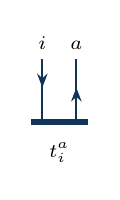
\begin{tikzpicture}[fcidiagram]
  \draw[amp] (-0.5,0) -- (0.5,0);
  \draw[hline] (-0.3,0) -- (-0.3,1.1); \draw[pline] (0.3,0) -- (0.3,1.1);
  \node[dlab,above] at (-0.3,1.1) {$i$}; \node[dlab,above] at (0.3,1.1) {$a$};
  \node[dlab,below] at (0,-0.2) {$t_i^a$};
\end{tikzpicture}
\hspace{3em}
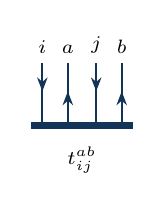
\begin{tikzpicture}[fcidiagram]
  \draw[amp] (-0.9,0) -- (0.9,0);
  \draw[hline] (-0.7,0) -- (-0.7,1.1); \draw[pline] (-0.25,0) -- (-0.25,1.1);
  \draw[hline] (0.25,0) -- (0.25,1.1); \draw[pline] (0.7,0) -- (0.7,1.1);
  \node[dlab,above] at (-0.7,1.1) {$i$}; \node[dlab,above] at (-0.25,1.1) {$a$};
  \node[dlab,above] at (0.25,1.1) {$j$}; \node[dlab,above] at (0.7,1.1) {$b$};
  \node[dlab,below] at (0,-0.2) {$t_{ij}^{ab}$};
\end{tikzpicture}
\par\small The amplitude bars of chapter 5 (week 38): in CC they are the unknowns; every open diagram of last week ends on bars like these.
\end{center}
\end{frame}

\begin{frame}[shrink=6]{Commuting excitations and the inverse cluster expansion}
Let $X_m$ and $X_n$ be pure excitation monomials of ranks $m,n$. Their single-fermion factors have zero mutual anticommutators: occupied and virtual labels belong to disjoint sets. Moving all $2m$ factors through all $2n$ factors gives
\[
 X_mX_n=(-1)^{(2m)(2n)}X_nX_m=X_nX_m.
\]
If a creation or annihilation label is repeated, both products vanish. Thus $[T_m,T_n]=0$, including overlapping excitations.
\medskip

For a state with nonzero reference overlap, impose intermediate normalisation and write $\ket{\Psi}=(1+C)\ket{\ph}$. The excitation algebra is nilpotent, so
\[
 T=\log(1+C)=C-\tfrac12C^2+\tfrac13C^3-\cdots
\]
is finite on the $N$-particle sector. In particular,
\[
 T_1=C_1,\quad T_2=C_2-\tfrac12C_1^2,\quad
 T_3=C_3-C_1C_2+\tfrac13C_1^3.
\]
Complete CI and complete CC are equivalent when this overlap is nonzero. Truncating $T$ retains products of lower-rank clusters, but omits independent higher-rank clusters.
\end{frame}

\begin{frame}[shrink=6]{Why exponentiate at all?}
\small
\[
e^{T}=1+T_1+\Bigl(T_2+\tfrac12T_1^2\Bigr)+\Bigl(T_3+T_1T_2+\tfrac16T_1^3\Bigr)+\Bigl(T_4+T_1T_3+\tfrac12T_2^2+\tfrac12T_1^2T_2+\tfrac1{24}T_1^4\Bigr)+\cdots
\]
Compare with CI, $\ket{\Psi}=(1+C_1+C_2+\cdots)\ket{\ph}$:
\[
C_1=T_1,\qquad C_2=T_2+\tfrac12T_1^2,\qquad C_3=T_3+T_1T_2+\tfrac16T_1^3,\qquad C_4\ni\tfrac12T_2^2 .
\]
\begin{itemize}
\item For nonzero reference overlap, complete $T$ and $C$ are equivalent. Each high-rank CI coefficient is an independent connected cluster plus products of lower-rank clusters. Truncating $T$ drops the independent higher clusters while retaining the products.
\item Truncate $C$ at doubles: the quadruples are gone, and a product of two doubles on separate subsystems \emph{is} a quadruple -- CID is not size consistent (week 38). Truncate $T$ at doubles: $\tfrac12T_2^2$ keeps it, with its amplitude fixed by the doubles.
\item Last week, ``disconnected but linked'': $\langle\Phi_{ijkl}^{abcd}|\Psi^{(2)}\rangle=t_mt_n$, a product of first-order doubles. That is $\tfrac12T_2^2$ at lowest order. The exponential generates every disconnected-but-linked diagram from the connected ones, and nothing else -- it is the wave-operator form of the theorem, $\Omega=[\,\cdot\,]_{\rm linked}$, as an ansatz.
\end{itemize}
\end{frame}

\begin{frame}{Pause to think \#1}
\thinkq{3}{Two non-interacting subsystems $A$ and $B$, reference $\ket{\ph}=\ket{\Phi_A}\ket{\Phi_B}$, no amplitude carries indices from both.
\begin{enumerate}
\item Show that $e^{T}\ket{\ph}=\bigl(e^{T_A}\ket{\Phi_A}\bigr)\bigl(e^{T_B}\ket{\Phi_B}\bigr)$. Which property of $T$ is used?
\item Show that $(1+C_2^A+C_2^B)\ket{\ph}$ is \emph{not} a product, and name the missing term.
\item What does 1.\ say about the energy of $A+B$ at any truncation of $T$?
\end{enumerate}}
\end{frame}

\begin{frame}{Answer to pause \#1}
\thinka{%
\begin{enumerate}
\item $T=T_A+T_B$ with $[T_A,T_B]=0$ (only $\cre{a}\ann{i}$ strings, on disjoint orbitals), so $e^{T}=e^{T_A}e^{T_B}$, and since the two act on disjoint orbitals the state factorises.
\item $(1+C_2^A)(1+C_2^B)=1+C_2^A+C_2^B+C_2^AC_2^B$: the cross term is a quadruple excitation, which CID has thrown away (section 5.9, week 38).
\item The energy of a product state under $H_A+H_B$ is $E_A+E_B$ -- at \emph{any} truncation, because $T_A$ and $T_B$ are truncated independently. Size extensivity is built in. With $T=T_2$: the quadruple $\tfrac12T_2^2$ is there, with its amplitude fixed by the doubles.
\end{enumerate}}
\end{frame}

\begin{frame}[shrink=7]{The similarity-transformed Hamiltonian}
Insert the ansatz in the Schr\"odinger equation and multiply from the left by $e^{-T}$ ($e^{T}$ is always invertible):
\[
 H e^{T}\ket{\ph}=Ee^{T}\ket{\ph}
 \quad\Longrightarrow\quad
 \boxed{\Hbar\ket{\ph}=E\ket{\ph},\qquad \Hbar=e^{-T}He^{T}.}
\]
\begin{itemize}
\item The reference determinant itself is asked to be an eigenstate -- of a transformed Hamiltonian. $H$ and $\Hbar$ have the same spectrum for \emph{any} $T$, truncated or not.
\item $T^\dagger\ne-T$: the transformation is not unitary and $\Hbar$ is not Hermitian. Left and right eigenvectors differ.
\item With $H=\Eref+H_N$: $\Hbar=\Eref+\Hbar_N$, $\Hbar_N=e^{-T}H_Ne^{T}$, and the energy relative to the reference is $\Delta E=E-\Eref$.
\end{itemize}
\begin{block}{Projecting}
\[
 \Delta E=\av{\Hbar_N},\qquad
 0=\mel{\Phi_i^a}{\Hbar_N}{\ph},\qquad
 0=\mel{\Phi_{ij}^{ab}}{\Hbar_N}{\ph},\qquad\dots
\]
One equation per amplitude. Truncating $T$ means keeping only the matching projections: the approximation is in the ansatz and in the restricted set of equations, not in the similarity identity.
\end{block}
\end{frame}

\begin{frame}[shrink=6]{Why the Baker-Campbell-Hausdorff series stops}
\small
\[
 \Hbar_N=H_N+[H_N,T]+\frac1{2!}[[H_N,T],T]+\frac1{3!}[[[H_N,T],T],T]+\frac1{4!}[[[[H_N,T],T],T],T]+\cdots
\]
Wick's theorem for a product of two normal-ordered strings (week 37): the product is the normal-ordered product plus all contractions \emph{between} the strings.
\begin{itemize}
\item $T$ contains only $\cre{a}$ (particle creation) and $\ann{i}$ (hole creation). Relative to $\ket{\ph}$ these are all quasi-particle \emph{creation} operators: there is no contraction between two $T$'s, and none with $T$ standing to the left of $H_N$.
\item Hence $H_NT=\no{H_NT}+(\text{contractions})$ while $TH_N=\no{TH_N}=\no{H_NT}$ (even number of operators, no sign). In the commutator the uncontracted product cancels:
\[
 [H_N,T]=\bigl(H_NT\bigr)_c\qquad\text{(at least one contraction between $H_N$ and $T$).}
\]
\item Each further commutator attaches one more $T$ to an operator of the original $H_N$. A two-body $H_N$ has four operators: at most four $T$'s.
\end{itemize}
\[
 \boxed{\Hbar_N=\Bigl(H_N\,e^{T}\Bigr)_c
 =\Bigl(H_N\bigl[1+T+\tfrac12T^2+\tfrac1{3!}T^3+\tfrac1{4!}T^4\bigr]\Bigr)_c}
\]
The subscript $c$: \emph{every} $T$ is contracted at least once with $H_N$. This is the linked-diagram theorem of week 46, now as an operator identity.
\end{frame}

\begin{frame}[shrink=19]{Coupled-cluster doubles: what is kept}
\[
 T=T_2=\frac14\sum_{ijab}t_{ij}^{ab}\,\cre a\cre b\ann j\ann i,\qquad
 t_{ij}^{ab}=-t_{ji}^{ab}=-t_{ij}^{ba}.
\]
One unknown per double excitation; the energy and the doubles projection:
\[
 \Delta E=\langle\bigl(H_Ne^{T_2}\bigr)_c\rangle,\qquad
 0=\mel{\Phi_{ij}^{ab}}{\bigl(H_Ne^{T_2}\bigr)_c}{\ph}.
\]
\begin{block}{How many powers of $T_2$ survive? Count operators}
$H_NT_2^{\,r}$ has (at most) $4+4r$ operators. The doubles projection leaves four uncontracted, the energy none; every contraction uses one operator of $H_N$.
\begin{center}
\begin{tabular}{lccc}
\toprule
 & operators left & contractions needed & allowed $r$\\
\midrule
energy & 0 & $2+2r\le4$ & $r=1$ ($r=0$: $\av{H_N}=0$)\\
doubles & 4 & $2r\le4$ & $r=0,1,2$\\
\bottomrule
\end{tabular}
\end{center}
\end{block}
\[
 \Delta E=\langle H_NT_2\rangle_c,\qquad
 0=\mel{\Phi_{ij}^{ab}}{\bigl(H_N[1+T_2+\tfrac12T_2^2]\bigr)_c}{\ph}\qquad\text{(exactly quadratic).}
\]
\end{frame}

\begin{frame}{Pause to think \#2}
\thinkq{3}{A similarity transformation preserves every eigenvalue, and CCD uses the exact $\Hbar=e^{-T_2}He^{T_2}$.
\begin{enumerate}
\item Why is the CCD energy then not the exact energy?
\item With $T=T_2$ and a two-body $H_N$: what is the largest particle rank (two-body, three-body, \dots) of an operator in $\Hbar_N$?
\item Which matrix elements of $\Hbar_N$ has CCD made zero, and which has it left alone?
\end{enumerate}}
\end{frame}

\begin{frame}{Answer to pause \#2}
\thinka{%
\begin{enumerate}
\item $E$ is an eigenvalue of $\Hbar$ only if $\Hbar\ket{\ph}=E\ket{\ph}$ holds in \emph{all} components. CCD imposes it on $\bra{\ph}$ and on the doubles $\bra{\Phi_{ij}^{ab}}$ only. Coupled cluster at a finite truncation is a similarity transformation \emph{plus} a projection, and the projection is where the approximation lives.
\item $H_N$ has four operators, each $T_2$ brings four and removes at least two by one contraction; with four $T_2$ attached by one contraction each, $4+16-8=12$ operators remain: up to \emph{six-body} terms.
\item Zero: the column $\mel{\Phi_{ij}^{ab}}{\Hbar_N}{\ph}$. Left alone: $\mel{\Phi_i^a}{\Hbar_N}{\ph}$ (singles: next week), triples, quadruples, \dots\ These residual couplings of the reference to other determinants are the whole error of CCD.
\end{enumerate}}
\end{frame}

\begin{frame}[shrink=6]{The road map for the rest of the week}
\small
\[
 0=\underbrace{\mel{\Phi_{ij}^{ab}}{H_N}{\ph}}_{\text{no }T}
 +\underbrace{\mel{\Phi_{ij}^{ab}}{(F_NT_2)_c}{\ph}+\mel{\Phi_{ij}^{ab}}{(V_NT_2)_c}{\ph}}_{\text{one }T}
 +\underbrace{\tfrac12\mel{\Phi_{ij}^{ab}}{(V_NT_2^2)_c}{\ph}}_{\text{two }T}
\]
\begin{center}
\renewcommand{\arraystretch}{1.25}
\begin{tabular}{llll}
\toprule
from & term & name & number of terms\\
\midrule
$H_N$ & $\as abij$ & driving term & 1\\
$F_NT_2$ & $P(ab)f_{bc}t_{ij}^{ac}-P(ij)f_{kj}t_{ik}^{ab}$ & Fock terms & 2\\
$V_NT_2$ & $\tfrac12\as abcd t_{ij}^{cd}$,\quad $\tfrac12\as klij t_{kl}^{ab}$ & pp and hh ladders & 2\\
$V_NT_2$ & $P(ij)P(ab)\as kbcj t_{ik}^{ac}$ & ring (particle-hole) & 1\\
$\tfrac12V_NT_2^2$ & four terms $\propto\as klcd\,t\,t$ & quadratic terms & 4\\
\bottomrule
\end{tabular}
\end{center}
\begin{itemize}
\item Thursday, lecture 2: all ten terms with Wick's theorem -- signs, factors $\tfrac12$ and $\tfrac14$, permutations.
\item Friday, lecture 3: all ten again as diagrams, each read off in one line.
\item Friday, lecture 4: all ten as one line of \texttt{numpy} each, for the pairing model.
\end{itemize}
($F_NT_2^2$ does not appear: a one-body operator has two operators and cannot reach two $T$'s and still leave a double.)
\end{frame}

% ======================================================================
\section[Thursday 2: CCD with Wick]{Thursday, lecture 2: The CCD equation from Wick's theorem}
% ======================================================================

\begin{frame}[shrink=10]{The toolbox: three facts from weeks 35--37}
\small
\begin{block}{1. Contractions relative to $\ket{\ph}$}
Only two are non-zero, and only with the operators in this order:
\[
 \ann a\,\cre b\ \to\ \delta_{ab}\quad(\text{particles}),\qquad\qquad
 \cre i\,\ann j\ \to\ \delta_{ij}\quad(\text{holes}).
\]
\end{block}
\begin{block}{2. The generalised Wick theorem}
$\no{A}\no{B}=\no{AB}+\sum(\text{all contractions between }A\text{ and }B)$; no contractions inside a normal-ordered string. A vacuum expectation value keeps only the fully contracted terms.
\end{block}
\begin{block}{3. The sign}
Contracting two operators that have $n$ operators between them costs $(-1)^n$ (move them next to each other first). Reordering inside $\no{\cdots}$ costs the sign of the permutation.
\end{block}
In $H_NT_2$, with $H_N$ on the left and $T_2\propto t_{kl}^{cd}\,\no{\cre c\cre d\ann l\ann k}$ on the right, the only possible contractions are therefore
\[
 \underbrace{\ann q\ \text{of}\ H_N\ \text{with}\ \cre c\ \text{of}\ T_2}_{\delta_{qc}:\ \text{a particle line}}
 \qquad\text{and}\qquad
 \underbrace{\cre p\ \text{of}\ H_N\ \text{with}\ \ann k\ \text{of}\ T_2}_{\delta_{pk}:\ \text{a hole line}} .
\]
\end{frame}

\begin{frame}[shrink=16]{A lemma that does the projection once and for all}
\small
\stepbox{Projection lemma}{For \emph{any} array $X_{kl}^{cd}$ (no symmetry assumed),
\[
 \mel{\Phi_{ij}^{ab}}{\sum_{klcd}X_{kl}^{cd}\,\no{\cre c\cre d\ann l\ann k}}{\ph}
 =X_{ij}^{ab}-X_{ji}^{ab}-X_{ij}^{ba}+X_{ji}^{ba}=P(ij)P(ab)\,X_{ij}^{ab}.
\]}
Proof. $\bra{\Phi_{ij}^{ab}}=\bra{\ph}\cre i\cre j\ann b\ann a$. Full contractions of
\begin{center}
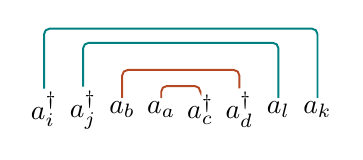
\begin{tikzpicture}[x=0.62cm,y=0.34cm,scale=1,baseline=(o0.base),every node/.style={inner sep=1.2pt,font=\normalsize}]
\node (o0) at (0.00,0) {$\cre i$};
\node (o1) at (1.00,0) {$\cre j$};
\node (o2) at (2.00,0) {$\ann b$};
\node (o3) at (3.00,0) {$\ann a$};
\node (o4) at (4.00,0) {$\cre c$};
\node (o5) at (5.00,0) {$\cre d$};
\node (o6) at (6.00,0) {$\ann l$};
\node (o7) at (7.00,0) {$\ann k$};
\draw[warm,line width=.7pt,rounded corners=2pt] (o3.north) -- ++(0,0.55) -| (o4.north);
\draw[warm,line width=.7pt,rounded corners=2pt] (o2.north) -- ++(0,1.30) -| (o5.north);
\draw[teal,line width=.7pt,rounded corners=2pt] (o1.north) -- ++(0,2.05) -| (o6.north);
\draw[teal,line width=.7pt,rounded corners=2pt] (o0.north) -- ++(0,2.80) -| (o7.north);
\end{tikzpicture}
$\;=+\,\delta_{ac}\delta_{bd}\delta_{jl}\delta_{ik}$
\end{center}
The pattern shown is nested (no crossings): sign $+$. Exchanging the two particle contractions gives one crossing, $-\delta_{ad}\delta_{bc}$; the same for the holes. Four patterns, four terms. \hfill$\square$
\begin{itemize}
\item If $X$ is antisymmetric in $(k,l)$ and in $(c,d)$ the four terms are equal: the result is $4X_{ij}^{ab}$. Check: $T_2=\tfrac14\sum t_{kl}^{cd}\no{\cdots}$ gives $\mel{\Phi_{ij}^{ab}}{T_2}{\ph}=t_{ij}^{ab}$.
\item If $X$ is antisymmetric in one pair only: $2P(ab)X_{ij}^{ab}$ or $2P(ij)X_{ij}^{ab}$.
\end{itemize}
\textbf{Strategy.} Contract $H_N$ with $T_2$ until a term of the form $\sum X_{kl}^{cd}\no{\cre c\cre d\ann l\ann k}$ is left. Read off the answer with the lemma. The permutation operators come out by themselves.
\end{frame}

\begin{frame}[shrink=16]{Warm-up 1: the energy}
\small
$\Delta E=\av{V_NT_2}$ ($F_N$ has only two operators and cannot close the four of $T_2$):
\[
 \Delta E=\frac14\cdot\frac14\sum_{pqrs}\sum_{klcd}\as pqrs\,t_{kl}^{cd}\,
 \av{\no{\cre p\cre q\ann s\ann r}\no{\cre c\cre d\ann l\ann k}} .
\]
All eight operators must be contracted: the annihilators $r,s$ with the particle creators $c,d$ and the creators $p,q$ with the hole operators $k,l$.
\begin{center}
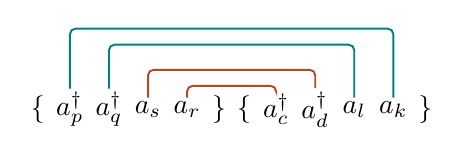
\begin{tikzpicture}[x=0.62cm,y=0.34cm,scale=1,baseline=(o0.base),every node/.style={inner sep=1.2pt,font=\normalsize}]
\node (o0) at (-0.18,0) {$\{$};
\node (o1) at (0.64,0) {$\cre p$};
\node (o2) at (1.64,0) {$\cre q$};
\node (o3) at (2.64,0) {$\ann s$};
\node (o4) at (3.64,0) {$\ann r$};
\node (o5) at (4.46,0) {$\}$};
\node (o6) at (5.10,0) {$\{$};
\node (o7) at (5.92,0) {$\cre c$};
\node (o8) at (6.92,0) {$\cre d$};
\node (o9) at (7.92,0) {$\ann l$};
\node (o10) at (8.92,0) {$\ann k$};
\node (o11) at (9.74,0) {$\}$};
\draw[warm,line width=.7pt,rounded corners=2pt] (o4.north) -- ++(0,0.55) -| (o7.north);
\draw[warm,line width=.7pt,rounded corners=2pt] (o3.north) -- ++(0,1.30) -| (o8.north);
\draw[teal,line width=.7pt,rounded corners=2pt] (o2.north) -- ++(0,2.05) -| (o9.north);
\draw[teal,line width=.7pt,rounded corners=2pt] (o1.north) -- ++(0,2.80) -| (o10.north);
\end{tikzpicture}
$\;=+\,\delta_{rc}\delta_{sd}\,\delta_{ql}\delta_{pk}$
\end{center}
Nested, sign $+$. Exchanging the particle contractions, or the hole contractions, gives a minus sign and exchanges two indices of $\as pqrs$, which gives another: all \textbf{four patterns are equal}.
\[
 \Delta E=\frac{4}{16}\sum_{klcd}\as klcd\,t_{kl}^{cd}
 \qquad\Longrightarrow\qquad
 \boxed{\Delta E=\frac14\sum_{ijab}\as ijab\,t_{ij}^{ab}}
\]
\begin{itemize}
\item The pattern of the whole derivation: prefactors $\times$ (number of equal contraction patterns). Here $\tfrac14\cdot\tfrac14\cdot4=\tfrac14$.
\item Same form as the CI correlation energy with $C_{ij}^{ab}\to t_{ij}^{ab}$, and the MBPT2 energy when $t\to\as abij/D_{ij}^{ab}$.
\end{itemize}
\end{frame}

\begin{frame}[shrink=3]{Warm-up 2: the driving term}
\small
No cluster operator: $\mel{\Phi_{ij}^{ab}}{H_N}{\ph}$. Only $V_N$ can create two particles and two holes.
\[
 \mel{\Phi_{ij}^{ab}}{V_N}{\ph}=\frac14\sum_{pqrs}\as pqrs\,
 \av{\cre i\cre j\ann b\ann a\,\no{\cre p\cre q\ann s\ann r}}
\]
\begin{center}
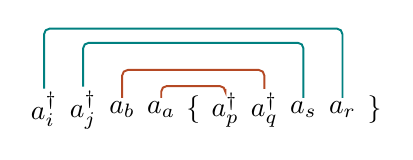
\begin{tikzpicture}[x=0.62cm,y=0.34cm,scale=1,baseline=(o0.base),every node/.style={inner sep=1.2pt,font=\normalsize}]
\node (o0) at (0.00,0) {$\cre i$};
\node (o1) at (1.00,0) {$\cre j$};
\node (o2) at (2.00,0) {$\ann b$};
\node (o3) at (3.00,0) {$\ann a$};
\node (o4) at (3.82,0) {$\{$};
\node (o5) at (4.64,0) {$\cre p$};
\node (o6) at (5.64,0) {$\cre q$};
\node (o7) at (6.64,0) {$\ann s$};
\node (o8) at (7.64,0) {$\ann r$};
\node (o9) at (8.46,0) {$\}$};
\draw[warm,line width=.7pt,rounded corners=2pt] (o3.north) -- ++(0,0.55) -| (o5.north);
\draw[warm,line width=.7pt,rounded corners=2pt] (o2.north) -- ++(0,1.30) -| (o6.north);
\draw[teal,line width=.7pt,rounded corners=2pt] (o1.north) -- ++(0,2.05) -| (o7.north);
\draw[teal,line width=.7pt,rounded corners=2pt] (o0.north) -- ++(0,2.80) -| (o8.north);
\end{tikzpicture}
$\;=+\,\delta_{ap}\delta_{bq}\,\delta_{js}\delta_{ir}$
\end{center}
Again four equal patterns: $\tfrac14\cdot4=1$.
\[
 \boxed{\mel{\Phi_{ij}^{ab}}{H_N}{\ph}=\as abij}
\]
\begin{itemize}
\item This is the Condon-Slater rule for a double excitation (week 37).
\item It is the only term without an amplitude: it \emph{drives} the equation. Without it $t=0$ is a solution. Keeping only this term and the diagonal Fock terms (next two frames) gives $t_{ij}^{ab}=\as abij/D_{ij}^{ab}$, the first-order wave function of week 44.
\end{itemize}
\end{frame}

\begin{frame}[shrink=10]{One $T_2$, one-body part: the particle Fock term}
\small
$F_NT_2=\tfrac14\sum f_{pq}t_{kl}^{cd}\no{\cre p\ann q}\no{\cre c\cre d\ann l\ann k}$. To leave a two-body operator: \textbf{one} contraction. First $\ann q$ with a particle:
\begin{center}
\begin{tabular}{@{}r@{\;\;}l@{}}
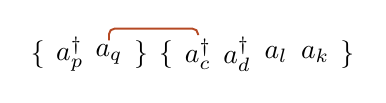
\begin{tikzpicture}[x=0.62cm,y=0.34cm,scale=1,baseline=(o0.base),every node/.style={inner sep=1.2pt,font=\normalsize}]
\node (o0) at (-0.18,0) {$\{$};
\node (o1) at (0.64,0) {$\cre p$};
\node (o2) at (1.64,0) {$\ann q$};
\node (o3) at (2.46,0) {$\}$};
\node (o4) at (3.10,0) {$\{$};
\node (o5) at (3.92,0) {$\cre c$};
\node (o6) at (4.92,0) {$\cre d$};
\node (o7) at (5.92,0) {$\ann l$};
\node (o8) at (6.92,0) {$\ann k$};
\node (o9) at (7.74,0) {$\}$};
\draw[warm,line width=.7pt,rounded corners=2pt] (o2.north) -- ++(0,0.55) -| (o5.north);
\end{tikzpicture} & $=+\,\delta_{qc}\no{\cre p\cre d\ann l\ann k}$\\[3pt]
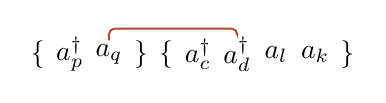
\begin{tikzpicture}[x=0.62cm,y=0.34cm,scale=1,baseline=(o0.base),every node/.style={inner sep=1.2pt,font=\normalsize}]
\node (o0) at (-0.18,0) {$\{$};
\node (o1) at (0.64,0) {$\cre p$};
\node (o2) at (1.64,0) {$\ann q$};
\node (o3) at (2.46,0) {$\}$};
\node (o4) at (3.10,0) {$\{$};
\node (o5) at (3.92,0) {$\cre c$};
\node (o6) at (4.92,0) {$\cre d$};
\node (o7) at (5.92,0) {$\ann l$};
\node (o8) at (6.92,0) {$\ann k$};
\node (o9) at (7.74,0) {$\}$};
\draw[warm,line width=.7pt,rounded corners=2pt] (o2.north) -- ++(0,0.55) -| (o6.north);
\end{tikzpicture} & $=-\,\delta_{qd}\no{\cre p\cre c\ann l\ann k}$
\end{tabular}
\end{center}
(one operator, $\cre c$, in between in the second). With $t_{kl}^{dc}=-t_{kl}^{cd}$ the two are equal:
\[
 \bigl(F_NT_2\bigr)_c\ \ni\ \frac12\sum f_{pc}\,t_{kl}^{cd}\,\no{\cre p\cre d\ann l\ann k}.
\]
A double excitation needs $p$ to be a particle, $p=e$. This has the form of the lemma with $X_{kl}^{ed}=\tfrac12\sum_cf_{ec}t_{kl}^{cd}$, antisymmetric in $(k,l)$ only:
\[
 2P(ab)X_{ij}^{ab}=P(ab)\sum_cf_{ac}\,t_{ij}^{cb}
 \qquad\Longrightarrow\qquad
 \boxed{+P(ab)\sum_cf_{bc}\,t_{ij}^{ac}}
\]
\begin{itemize}
\item $P(ab)$ appears because the Fock operator sits on one of two particle lines: $a$ and $b$ are no longer equivalent.
\item Weight: $\tfrac14$ (from $T_2$) $\times\,2$ (equal patterns) $\times\,2$ (lemma) $=1$ per term.
\end{itemize}
\end{frame}

\begin{frame}[shrink=16]{One $T_2$, one-body part: the hole Fock term}
\small
Now contract $\cre p$ with a hole operator of $T_2$:
\begin{center}
\begin{tabular}{@{}r@{\;\;}l@{}}
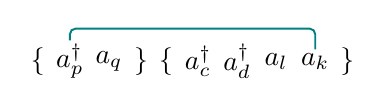
\begin{tikzpicture}[x=0.62cm,y=0.34cm,scale=1,baseline=(o0.base),every node/.style={inner sep=1.2pt,font=\normalsize}]
\node (o0) at (-0.18,0) {$\{$};
\node (o1) at (0.64,0) {$\cre p$};
\node (o2) at (1.64,0) {$\ann q$};
\node (o3) at (2.46,0) {$\}$};
\node (o4) at (3.10,0) {$\{$};
\node (o5) at (3.92,0) {$\cre c$};
\node (o6) at (4.92,0) {$\cre d$};
\node (o7) at (5.92,0) {$\ann l$};
\node (o8) at (6.92,0) {$\ann k$};
\node (o9) at (7.74,0) {$\}$};
\draw[teal,line width=.7pt,rounded corners=2pt] (o1.north) -- ++(0,0.55) -| (o8.north);
\end{tikzpicture} & $=+\,\delta_{pk}\no{\ann q\cre c\cre d\ann l}$\\[3pt]
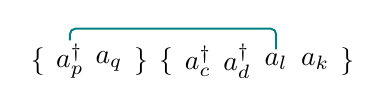
\begin{tikzpicture}[x=0.62cm,y=0.34cm,scale=1,baseline=(o0.base),every node/.style={inner sep=1.2pt,font=\normalsize}]
\node (o0) at (-0.18,0) {$\{$};
\node (o1) at (0.64,0) {$\cre p$};
\node (o2) at (1.64,0) {$\ann q$};
\node (o3) at (2.46,0) {$\}$};
\node (o4) at (3.10,0) {$\{$};
\node (o5) at (3.92,0) {$\cre c$};
\node (o6) at (4.92,0) {$\cre d$};
\node (o7) at (5.92,0) {$\ann l$};
\node (o8) at (6.92,0) {$\ann k$};
\node (o9) at (7.74,0) {$\}$};
\draw[teal,line width=.7pt,rounded corners=2pt] (o1.north) -- ++(0,0.55) -| (o7.north);
\end{tikzpicture} & $=-\,\delta_{pl}\no{\ann q\cre c\cre d\ann k}$
\end{tabular}
\end{center}
(four operators in between, then three). Equal by $t_{lk}^{cd}=-t_{kl}^{cd}$:
\[
 \bigl(F_NT_2\bigr)_c\ \ni\ \frac12\sum f_{kq}\,t_{kl}^{cd}\,\no{\ann q\cre c\cre d\ann l}
 =\alert{-}\frac12\sum f_{km}\,t_{kl}^{cd}\,\no{\cre c\cre d\ann l\ann m}.
\]
For a double excitation $q=m$ is a hole, and bringing $\ann m$ to its place at the right end moves it past three operators: \alert{a minus sign}. Lemma with $X_{ml}^{cd}=-\tfrac12\sum_kf_{km}t_{kl}^{cd}$, antisymmetric in $(c,d)$:
\[
 2P(ij)X_{ij}^{ab}=-P(ij)\sum_kf_{ki}\,t_{kj}^{ab}
 \qquad\Longrightarrow\qquad
 \boxed{-P(ij)\sum_kf_{kj}\,t_{ik}^{ab}}
\]
\begin{itemize}
\item The sign is the first instance of a general rule we shall read off diagrams tomorrow: every hole line costs a factor $-1$.
\item Two contractions between $F_N$ and $T_2$ leave a one-body operator, $\sum f_{kc}t_{kl}^{cd}\no{\cre d\ann l}$: it contributes to the \emph{singles} projection, not to ours.
\end{itemize}
\end{frame}

\begin{frame}[shrink=7]{The Fock terms contain the energy denominators}
Split $f=f^{\rm d}+f'$ into its diagonal and off-diagonal parts. The diagonal part of the two Fock terms is
\[
 P(ab)f_{bb}t_{ij}^{ab}-P(ij)f_{jj}t_{ij}^{ab}
 =\bigl(f_{aa}+f_{bb}-f_{ii}-f_{jj}\bigr)t_{ij}^{ab}\equiv-D_{ij}^{ab}\,t_{ij}^{ab},
\]
\[
 D_{ij}^{ab}=f_{ii}+f_{jj}-f_{aa}-f_{bb}=\varepsilon_i+\varepsilon_j-\varepsilon_a-\varepsilon_b\ <0 .
\]
\begin{block}{The equation so far}
\[
 0=\as abij-D_{ij}^{ab}t_{ij}^{ab}+P(ab)f'_{bc}t_{ij}^{ac}-P(ij)f'_{kj}t_{ik}^{ab}+\bigl(V_NT_2\bigr)+\tfrac12\bigl(V_NT_2^2\bigr)
\]
\end{block}
\begin{itemize}
\item Nobody put a resolvent into coupled-cluster theory. The denominators of perturbation theory are the diagonal Fock terms of $[H_N,T_2]$, moved to the other side: $D\,t=\as abij+\cdots$.
\item In a canonical Hartree-Fock basis $f'=0$ and the Fock terms are \emph{only} the denominators. For the pairing model $f$ is diagonal as well.
\item The split is a choice (a preconditioner for the iteration), not physics: the equation does not know about it.
\end{itemize}
\end{frame}

\begin{frame}[shrink=3]{One $T_2$, two-body part: how many contractions?}
\small
$V_NT_2=\tfrac1{16}\sum\as pqrs\,t_{kl}^{cd}\no{\cre p\cre q\ann s\ann r}\no{\cre c\cre d\ann l\ann k}$ has eight operators. Each contraction removes two.
\begin{center}
\renewcommand{\arraystretch}{1.3}
\begin{tabular}{clll}
\toprule
contractions & what is left & contributes to & this week?\\
\midrule
1 & six operators: a three-body operator & triples projection & no\\
\textbf{2} & \textbf{four operators: a two-body operator} & \textbf{doubles projection} & \textbf{yes}\\
3 & two operators: a one-body operator & singles projection & no (CCSD)\\
4 & a number & the energy & done\\
\bottomrule
\end{tabular}
\end{center}
Two contractions, each either a particle line or a hole line: three possibilities.
\begin{center}
\renewcommand{\arraystretch}{1.2}
\begin{tabular}{lll}
\toprule
lines between $V_N$ and $T_2$ & block of $V_N$ that is needed & name\\
\midrule
two particle lines & $\as abcd$ & particle-particle ladder\\
two hole lines & $\as klij$ & hole-hole ladder\\
one particle, one hole line & $\as kbcj$ & ring (particle-hole)\\
\bottomrule
\end{tabular}
\end{center}
The lines that are \emph{not} contracted must be two particle creators and two hole creators (the lemma), which fixes the block of $V_N$ in each case.
\end{frame}

\begin{frame}[shrink=12]{The particle-particle ladder}
\small
Contract both annihilators of $V_N$ with the two particle creators of $T_2$:
\begin{center}
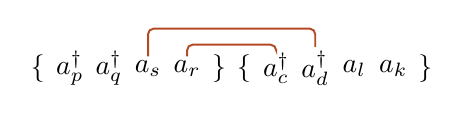
\begin{tikzpicture}[x=0.62cm,y=0.34cm,scale=1,baseline=(o0.base),every node/.style={inner sep=1.2pt,font=\normalsize}]
\node (o0) at (-0.18,0) {$\{$};
\node (o1) at (0.64,0) {$\cre p$};
\node (o2) at (1.64,0) {$\cre q$};
\node (o3) at (2.64,0) {$\ann s$};
\node (o4) at (3.64,0) {$\ann r$};
\node (o5) at (4.46,0) {$\}$};
\node (o6) at (5.10,0) {$\{$};
\node (o7) at (5.92,0) {$\cre c$};
\node (o8) at (6.92,0) {$\cre d$};
\node (o9) at (7.92,0) {$\ann l$};
\node (o10) at (8.92,0) {$\ann k$};
\node (o11) at (9.74,0) {$\}$};
\draw[warm,line width=.7pt,rounded corners=2pt] (o4.north) -- ++(0,0.55) -| (o7.north);
\draw[warm,line width=.7pt,rounded corners=2pt] (o3.north) -- ++(0,1.30) -| (o8.north);
\end{tikzpicture}
$=+\delta_{rc}\delta_{sd}\no{\cre p\cre q\ann l\ann k}$,\qquad crossed: $-\delta_{rd}\delta_{sc}\no{\cre p\cre q\ann l\ann k}$
\end{center}
Equal, since $\as pqdc=-\as pqcd$. Two equal patterns:
\[
 \bigl(V_NT_2\bigr)_c\ \ni\ \frac{2}{16}\sum\as efcd\,t_{kl}^{cd}\,\no{\cre e\cre f\ann l\ann k}
 \qquad(p,q\to\text{particles }e,f).
\]
Lemma with $X_{kl}^{ef}=\tfrac18\sum_{cd}\as efcd t_{kl}^{cd}$, antisymmetric in both pairs: $4X_{ij}^{ab}$,
\[
 \boxed{+\frac12\sum_{cd}\as abcd\,t_{ij}^{cd}}
\]
\begin{itemize}
\item The two particles excited by $T_2$ scatter once more into $a,b$; the holes $i,j$ are spectators.
\item The factor $\tfrac12$: the two particle lines $c,d$ run between the same two operators and are \emph{equivalent} -- summing freely over $c$ and $d$ counts each pair twice.
\item No permutation operator: $a,b$ leave from the same operator ($V_N$), and so do $i,j$ ($T_2$). The term is already antisymmetric.
\end{itemize}
\end{frame}

\begin{frame}{The hole-hole ladder}
\small
Contract both creators of $V_N$ with the two hole operators of $T_2$:
\begin{center}
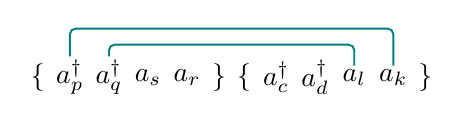
\begin{tikzpicture}[x=0.62cm,y=0.34cm,scale=1,baseline=(o0.base),every node/.style={inner sep=1.2pt,font=\normalsize}]
\node (o0) at (-0.18,0) {$\{$};
\node (o1) at (0.64,0) {$\cre p$};
\node (o2) at (1.64,0) {$\cre q$};
\node (o3) at (2.64,0) {$\ann s$};
\node (o4) at (3.64,0) {$\ann r$};
\node (o5) at (4.46,0) {$\}$};
\node (o6) at (5.10,0) {$\{$};
\node (o7) at (5.92,0) {$\cre c$};
\node (o8) at (6.92,0) {$\cre d$};
\node (o9) at (7.92,0) {$\ann l$};
\node (o10) at (8.92,0) {$\ann k$};
\node (o11) at (9.74,0) {$\}$};
\draw[teal,line width=.7pt,rounded corners=2pt] (o2.north) -- ++(0,0.55) -| (o9.north);
\draw[teal,line width=.7pt,rounded corners=2pt] (o1.north) -- ++(0,1.30) -| (o10.north);
\end{tikzpicture}
$=+\delta_{ql}\delta_{pk}\no{\ann s\ann r\cre c\cre d}$
\end{center}
(six operators between $\cre q$ and $\ann l$; then six between $\cre p$ and $\ann k$). The crossed pattern is again equal. With $r,s\to$ holes $m,n$ and $\no{\ann n\ann m\cre c\cre d}=+\no{\cre c\cre d\ann n\ann m}$ (two operators past two):
\[
 \bigl(V_NT_2\bigr)_c\ \ni\ \frac{2}{16}\sum\as klmn\,t_{kl}^{cd}\,\no{\cre c\cre d\ann n\ann m}
 \qquad\Longrightarrow\qquad
 \boxed{+\frac12\sum_{kl}\as klij\,t_{kl}^{ab}}
\]
\begin{itemize}
\item Mirror image of the previous frame: the two holes scatter, the particles watch. Two hole lines, two minus signs: $+$.
\item Iterated, the two ladder terms sum the particle-particle and hole-hole ladder diagrams of perturbation theory to all orders; the third-order ladders of week 45 are the first rung.
\end{itemize}
\end{frame}

\begin{frame}[shrink=16]{The ring (particle-hole) term}
\small
One particle contraction and one hole contraction. A representative pattern:
\begin{center}
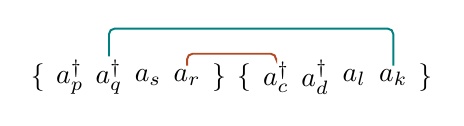
\begin{tikzpicture}[x=0.62cm,y=0.34cm,scale=1,baseline=(o0.base),every node/.style={inner sep=1.2pt,font=\normalsize}]
\node (o0) at (-0.18,0) {$\{$};
\node (o1) at (0.64,0) {$\cre p$};
\node (o2) at (1.64,0) {$\cre q$};
\node (o3) at (2.64,0) {$\ann s$};
\node (o4) at (3.64,0) {$\ann r$};
\node (o5) at (4.46,0) {$\}$};
\node (o6) at (5.10,0) {$\{$};
\node (o7) at (5.92,0) {$\cre c$};
\node (o8) at (6.92,0) {$\cre d$};
\node (o9) at (7.92,0) {$\ann l$};
\node (o10) at (8.92,0) {$\ann k$};
\node (o11) at (9.74,0) {$\}$};
\draw[warm,line width=.7pt,rounded corners=2pt] (o4.north) -- ++(0,0.55) -| (o7.north);
\draw[teal,line width=.7pt,rounded corners=2pt] (o2.north) -- ++(0,1.30) -| (o10.north);
\end{tikzpicture}
$=-\,\delta_{rc}\delta_{qk}\no{\cre p\ann s\cre d\ann l}$
\end{center}
($\ann r\cre c$ adjacent: $+$; then $\cre q$ and $\ann k$ have $\ann s,\cre d,\ann l$ between them: $-$.) There are $2\times2$ choices for the particle contraction and $2\times2$ for the hole contraction; by the antisymmetry of $\as pqrs$ and $t_{kl}^{cd}$ all \textbf{16 patterns are equal}: $16/16=1$.

A double excitation needs $p=e$ (particle), $s=m$ (hole); $\no{\cre e\ann m\cre d\ann l}=+\no{\cre e\cre d\ann l\ann m}$:
\[
 \bigl(V_NT_2\bigr)_c\ \ni\ -\sum\as ekcm\,t_{kl}^{cd}\,\no{\cre e\cre d\ann l\ann m},
 \qquad X_{ml}^{ed}=-\sum_{kc}\as ekcm\,t_{kl}^{cd}.
\]
This $X$ has no symmetry, so the lemma gives all four terms:
\[
 -P(ij)P(ab)\sum_{kc}\as akci\,t_{kj}^{cb}
 \qquad\Longrightarrow\qquad
 \boxed{+P(ij)P(ab)\sum_{kc}\as kbcj\,t_{ik}^{ac}}
\]
(relabel $i\leftrightarrow j$, $a\leftrightarrow b$ under the permutations, then $\as bkcj=-\as kbcj$, $t_{ki}^{ca}=t_{ik}^{ac}$).
\begin{itemize}
\item One particle-hole pair of $T_2$ is annihilated and re-created as $(b,j)$; the other pair $(a,i)$ passes through. Iterated: the ring diagrams of RPA (chapter 7).
\item No $\tfrac12$ (the two lines are of different kind), but the full $P(ij)P(ab)$.
\end{itemize}
\end{frame}

\begin{frame}{Pause to think \#3}
\thinkq{4}{The three two-body terms came out with weights $\tfrac12$, $\tfrac12$ and $1$.
\begin{enumerate}
\item For each of them: how many \emph{complete} contraction patterns of
$\av{\cre i\cre j\ann b\ann a\,\no{\cre p\cre q\ann s\ann r}\no{\cre c\cre d\ann l\ann k}}$ are there (include the contractions with the bra)? Compare with the prefactor $\tfrac1{16}$.
\item State a rule for when a factor $\tfrac12$ appears, and a rule for when $P(ij)$ or $P(ab)$ appears.
\end{enumerate}}
\end{frame}

\begin{frame}{Answer to pause \#3}
\thinka{\normalsize%
\begin{center}
\renewcommand{\arraystretch}{1.25}
\begin{tabular}{lcccc}
\toprule
 & $V_N$--$T_2$ & bra--rest & patterns$/16$ & distinct terms $\times$ weight\\
\midrule
pp ladder & $2$ & $2\cdot2$ & $8/16$ & $1\times\tfrac12$\\
hh ladder & $2$ & $2\cdot2$ & $8/16$ & $1\times\tfrac12$\\
ring & $4\cdot4$ & $2\cdot2$ & $64/16$ & $4\times1$\\
\bottomrule
\end{tabular}
\end{center}
\begin{enumerate}
\item Ladders: the two annihilators (creators) of $V_N$ meet the two particles (holes) of $T_2$ in $2$ ways; the bra meets the remaining particles and holes in $2\cdot2$ ways. All eight give the \emph{same} term. Ring: $64$ patterns, falling into four classes of $16$ -- the four terms of $P(ij)P(ab)$.
\item $\tfrac12$ for each pair of \textbf{equivalent internal lines}: same kind, joining the same two operators. $P(ab)$ [or $P(ij)$] whenever the two \textbf{external} particle [hole] lines leave from \emph{different} operators, so that exchanging them gives a different term.
\end{enumerate}
These are two of tomorrow's diagram rules; the third is the sign.}
\end{frame}

\begin{frame}[shrink=3]{Two $T_2$: contract, then contract again}
\small
$\tfrac12[[V_N,T_2],T_2]$: the second $T_2$ contracts with what the first one left of $V_N$ -- never with the first $T_2$. Twelve operators, four must remain: \textbf{four contractions}, so \emph{all four} operators of $V_N$ are used. The only block that can send two hole lines and two particle lines \emph{down} into amplitudes is
\[
 \as klcd:\qquad \cre k,\cre l\ \text{contract with hole operators,}\quad \ann c,\ann d\ \text{with particle creators.}
\]
What distinguishes the terms is how the four lines $k,l,c,d$ are shared between the two amplitudes $T_A$ and $T_B$:
\begin{center}
\renewcommand{\arraystretch}{1.3}
\begin{tabular}{lllc}
\toprule
$T_A$ takes & $T_B$ takes & structure & name\\
\midrule
$c,d$ (two particles) & $k,l$ (two holes) & $2+2$ & $Q_a$\\
$k,c$ (hole, particle) & $l,d$ (hole, particle) & $2+2$ & $Q_b$\\
$c$ (one particle) & $k,l,d$ & $1+3$ & $Q_c$\\
$k$ (one hole) & $l,c,d$ & $1+3$ & $Q_d$\\
\midrule
nothing & $k,l,c,d$ & $0+4$ & \alert{not connected}\\
\bottomrule
\end{tabular}
\end{center}
Four connected terms. The last row has $T_A$ attached to nothing: it cannot arise from a commutator. We return to it in two frames -- it is the most instructive of the five.
\end{frame}

\begin{frame}[shrink=13]{The quadratic terms are the linear terms with dressed vertices}
\small
Contract $T_B$ with $V_N$ first. What is left is an operator with amplitudes inside -- a \emph{dressed} vertex (an intermediate):
\begin{center}
\renewcommand{\arraystretch}{1.45}
\begin{tabular}{llll}
\toprule
$T_B$ takes & operator left & intermediate & behaves like\\
\midrule
$k,l,d$ & $\sum\chi_{cb}\no{\cre b\ann c}$ & $\chi_{cb}=-\tfrac12\sum_{kld}\as klcd\,t_{kl}^{bd}$ & $f_{bc}$\\
$l,c,d$ & $\sum\chi_{kj}\no{\cre k\ann j}$ & $\chi_{kj}=+\tfrac12\sum_{lcd}\as klcd\,t_{jl}^{cd}$ & $f_{kj}$\\
$c,d$ & two-body, hole-hole & $\chi_{klij}=\tfrac12\sum_{cd}\as klcd\,t_{ij}^{cd}$ & $\as klij$\\
$l,d$ & two-body, particle-hole & $\chi_{bkcj}=\tfrac12\sum_{ld}\as klcd\,t_{lj}^{db}$ & $\as kbcj$\\
\bottomrule
\end{tabular}
\end{center}
Then contract $T_A$ exactly as on the previous frames:
\begin{align*}
 Q_c&=P(ab)\,\chi_{cb}\,t_{ij}^{ac}=-\tfrac12P(ab)\as klcd\,t_{ij}^{ac}t_{kl}^{bd},&
 Q_d&=-P(ij)\,\chi_{kj}\,t_{ik}^{ab}=-\tfrac12P(ij)\as klcd\,t_{ik}^{ab}t_{jl}^{cd},\\
 Q_a&=\tfrac12\,\chi_{klij}\,t_{kl}^{ab}=\tfrac14\as klcd\,t_{ij}^{cd}t_{kl}^{ab},&
 Q_b&=P(ij)P(ab)\,\chi_{bkcj}\,t_{ik}^{ac}=\tfrac12P(ij)P(ab)\as klcd\,t_{ik}^{ac}t_{jl}^{bd}.
\end{align*}
\begin{itemize}
\item The $\tfrac12$ of $e^{T}$: in $Q_a,Q_c,Q_d$ the two amplitudes play different roles, and either can play either role -- a factor $2$ cancels it. In $Q_b$ they play the same role: the $\tfrac12$ stays.
\item The remaining $\tfrac12$'s are equivalent lines: $(k,l)$ in $\chi_{cb}$, $(c,d)$ in $\chi_{kj}$ and $\chi_{klij}$, $(k,l)$ once more in $Q_a$.
\end{itemize}
\end{frame}

\begin{frame}[shrink=13]{The fifth distribution: where the energy went}
\small
Without the subscript $c$, $\tfrac12\mel{\Phi_{ij}^{ab}}{V_NT_2^2}{\ph}$ also contains the pattern in which one amplitude takes all four lines of $V_N$ and the other goes straight to the bra:
\[
 \tfrac12\mel{\Phi_{ij}^{ab}}{V_NT_2^2}{\ph}
 =\underbrace{\Bigl(\tfrac14\sum\as klcd\,t_{kl}^{cd}\Bigr)}_{\Delta E}\,t_{ij}^{ab}+Q_a+Q_b+Q_c+Q_d .
\]
In $\Hbar_N=e^{-T_2}H_Ne^{T_2}$ the term $-T_2H_NT_2$ of the commutators removes it: $-\mel{\Phi_{ij}^{ab}}{T_2V_NT_2}{\ph}=-t_{ij}^{ab}\,\Delta E$.
\begin{block}{Configuration interaction versus coupled cluster, in one line each}
\begin{align*}
\text{CID:}\quad 0&=\as abij+(\text{Fock, ladders, ring})[C]\ \alert{-\,\Delta E\,C_{ij}^{ab}}\\
\text{CCD:}\quad 0&=\as abij+(\text{Fock, ladders, ring})[t]\ \alert{+\,Q_a+Q_b+Q_c+Q_d}
\end{align*}
\end{block}
\begin{itemize}
\item CID has no quadruples: it keeps the disconnected term $-\Delta E\,C$, an energy times an amplitude, which grows with the size of the system. This is the lack of size extensivity of week 38, seen in the equation.
\item CCD includes the quadruples $\tfrac12T_2^2$: their disconnected part cancels $-\Delta E\,t$ \emph{exactly}, and what is left is connected.
\item At lowest order $-\Delta E\,t$ is the folded term $-E^{(2)}\as abij/D$ of week 46.
\end{itemize}
\end{frame}

\begin{frame}{Pause to think \#4}
\thinkq{4}{Take a system with only \emph{two} particles, so that $T_2^2\ket{\ph}=0$: there are no quadruples.
\begin{enumerate}
\item Does that mean $Q_a+Q_b+Q_c+Q_d=0$? Use the previous frame.
\item What does the CCD equation become, and what does that say about the accuracy of CCD for two particles (say, one pair in the pairing model)?
\item Now take $M$ such pairs, far apart and not interacting. Which of CID and CCD is exact?
\end{enumerate}}
\end{frame}

\begin{frame}[shrink=1]{Answer to pause \#4}
\thinka{%
\begin{enumerate}
\item No. The left-hand side $\tfrac12\mel{\Phi_{ij}^{ab}}{V_NT_2^2}{\ph}$ vanishes, hence $Q_a+Q_b+Q_c+Q_d=-\Delta E\,t_{ij}^{ab}$. The connected terms are individually non-zero and add up to minus the disconnected one. (Notebook: true to $10^{-17}$ for a random two-particle Hamiltonian.)
\item The CCD equation \emph{is} the CID equation. For two particles CID is the full CI in the space without singles: CCD is exact whenever singles are absent, e.g.\ one pair in the pairing model ($-0.6180339887$ for two levels, $g=1$, both ways).
\item CCD. With $T=\sum_AT_2^{A}$ the equations decouple into $M$ copies of the two-particle problem, each solved exactly, and the energies add. CID lacks the products $C_2^AC_2^B$ and is exact for $M=1$ only.
\end{enumerate}
Coupled-cluster doubles is \emph{exact for any number of independent pairs}. This is the content of the old name ``coupled-pair many-electron theory'' (\v{C}\'i\v{z}ek 1966).}
\end{frame}

\begin{frame}[shrink=10]{The CCD amplitude equation, complete}
\small
\begin{align*}
0={}&\underbrace{\as abij}_{\text{driving}}
 +\underbrace{P(ab)f_{bc}t_{ij}^{ac}-P(ij)f_{kj}t_{ik}^{ab}}_{\text{Fock terms (diagonal part: }-D_{ij}^{ab}t_{ij}^{ab})}
 +\underbrace{\tfrac12\as abcd\,t_{ij}^{cd}}_{\text{pp ladder}}
 +\underbrace{\tfrac12\as klij\,t_{kl}^{ab}}_{\text{hh ladder}}
 +\underbrace{P(ij)P(ab)\as kbcj\,t_{ik}^{ac}}_{\text{ring}}\\[2pt]
 &+\underbrace{\tfrac14\as klcd\,t_{ij}^{cd}t_{kl}^{ab}}_{Q_a}
 +\underbrace{\tfrac12P(ij)P(ab)\as klcd\,t_{ik}^{ac}t_{jl}^{bd}}_{Q_b}
 \underbrace{-\tfrac12P(ab)\as klcd\,t_{ij}^{ac}t_{kl}^{bd}}_{Q_c}
 \underbrace{-\tfrac12P(ij)\as klcd\,t_{ik}^{ab}t_{jl}^{cd}}_{Q_d}
\end{align*}
\[
 \Delta E=\frac14\sum_{ijab}\as ijab\,t_{ij}^{ab}
\]
One equation for each of the $n_o^2n_v^2$ amplitudes; ten terms; quadratic. Nothing has been neglected beyond $T=T_2$ and the choice of projections. Checked in \texttt{week47.ipynb} against $\mel{\Phi_{ij}^{ab}}{e^{-T_2}He^{T_2}}{\ph}$ built by brute force in the space of determinants (random Hamiltonian, non-diagonal Fock matrix, random amplitudes):
\numbox{No $T$, one $T$, two $T$'s, compared with $H$, $[H,T]$, $\tfrac12[[H,T],T]$: largest differences $0$, $9\times10^{-15}$, $4\times10^{-15}$. Triple commutator on doubles: $0$.}
\end{frame}

\begin{frame}[shrink=3]{Summary of Thursday}
\begin{itemize}
\item $\ket{\Psi}=e^{T}\ket{\ph}$ turns the Schr\"odinger equation into $\Hbar\ket{\ph}=E\ket{\ph}$ with $\Hbar_N=(H_Ne^{T})_c$: a finite, connected expansion.
\item CCD: $T=T_2$, the energy and the doubles projection. Operator counting limits the doubles equation to $T_2^2$.
\item Each term is (prefactors) $\times$ (number of equal contraction patterns), with
\begin{itemize}
\item $\tfrac12$ for each pair of equivalent internal lines,
\item $P(ij)$, $P(ab)$ for external lines leaving different operators,
\item a sign from the reordering -- a minus for each hole line pulled through (to be made precise tomorrow).
\end{itemize}
\item The diagonal Fock terms are the energy denominators. The ladders and the ring are the three ways a two-body vertex can touch an amplitude twice.
\item The four quadratic terms are the Fock, hole-hole and ring terms once more with dressed vertices; the fifth, disconnected distribution $\Delta E\,t$ cancels. That cancellation is what CID lacks.
\end{itemize}
\vspace{0.3em}
\small Tomorrow: every boxed formula of today read off a picture in one line, and then the whole equation as code.
\end{frame}

% ======================================================================
\section[Friday 3: CCD with diagrams]{Friday, lecture 3: The CCD equation from diagrams}
% ======================================================================

\begin{frame}[shrink=13]{From contraction patterns to pictures}
\small
Yesterday every term was (prefactors) $\times$ (number of equal contraction patterns) $\times$ (a sign). A diagram is a picture of one class of equal patterns, and the rules of week 45 turn the three ingredients into three glances.
\begin{center}
\renewcommand{\arraystretch}{1.35}
\begin{tabular}{ll}
\toprule
Wick's theorem (Thursday) & diagram (today)\\
\midrule
operator $\no{\cre p\cre q\ann s\ann r}$ with $\as pqrs$ & dashed interaction line, two vertices\\
operator $\no{\cre p\ann q}$ with $f_{pq}$ & a cross\\
$T_2$ with $t_{ij}^{ab}$ & a horizontal bar with two vertices\\
contraction $\ann q\cre c\to\delta_{qc}$ & particle line (arrow up) from bar to vertex\\
contraction $\cre p\ann k\to\delta_{pk}$ & hole line (arrow down) from bar to vertex\\
uncontracted operators, closed by $\bra{\Phi_{ij}^{ab}}$ & open (external) lines at the top\\
number of equal patterns $\times$ prefactors & $\tfrac12$ per pair of equivalent lines or vertices\\
the four terms of the lemma & $P(ij)$, $P(ab)$ for inequivalent external lines\\
sign from reordering & $(-1)^{h+l}$: hole lines and loops\\
\bottomrule
\end{tabular}
\end{center}
Time runs upwards. Because $\Hbar_N=(H_Ne^{T})_c$ has every $T$ to the right of $H_N$, the bars are always at the bottom and the one $H_N$ vertex on top. There are \textbf{no denominators}: the resolvents of perturbation theory are inside the amplitudes.
\end{frame}

\begin{frame}[shrink=13]{The elements: fragments of $H_N$ and their excitation level}
\small
\begin{center}
\begin{tabular}{@{}c@{\hspace{1.3em}}c@{\hspace{1.3em}}c@{\hspace{1.3em}}c@{\hspace{2.2em}}c@{\hspace{2.2em}}c@{\hspace{1.3em}}c@{\hspace{1.3em}}c@{}}
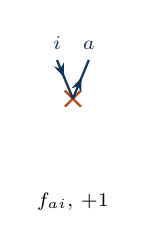
\begin{tikzpicture}[fcidiagram,baseline={(0,0)},scale=0.85]
    \node[fvtx] (h0) at (0.00,1.35) {};
    \draw[pline] (h0.center) -- (0.33,2.15) node[dlab,above] {$a$};
    \draw[hline] (h0.center) -- (-0.33,2.15) node[dlab,above] {$i$};
    \node[dlab,below] at (0.00,-0.40) {$f_{ai}$, $+1$};
\end{tikzpicture} & 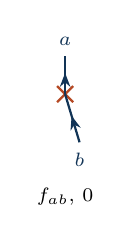
\begin{tikzpicture}[fcidiagram,baseline={(0,0)},scale=0.85]
    \node[fvtx] (h0) at (0.00,1.35) {};
    \draw[pline] (h0.center) -- (0.00,2.15) node[dlab,above] {$a$};
    \draw[pline] (0.30,0.35) node[dlab,below] {$b$} -- (h0.center);
    \node[dlab,below] at (0.00,-0.40) {$f_{ab}$, $0$};
\end{tikzpicture} & 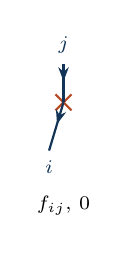
\begin{tikzpicture}[fcidiagram,baseline={(0,0)},scale=0.85]
    \node[fvtx] (h0) at (0.00,1.35) {};
    \draw[hline] (-0.30,0.35) node[dlab,below] {$i$} -- (h0.center);
    \draw[hline] (h0.center) -- (0.00,2.15) node[dlab,above] {$j$};
    \node[dlab,below] at (0.00,-0.40) {$f_{ij}$, $0$};
\end{tikzpicture} & 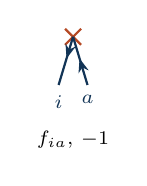
\begin{tikzpicture}[fcidiagram,baseline={(0,0)},scale=0.85]
    \node[fvtx] (h0) at (0.00,1.35) {};
    \draw[hline] (-0.30,0.35) node[dlab,below] {$i$} -- (h0.center);
    \draw[pline] (0.30,0.35) node[dlab,below] {$a$} -- (h0.center);
    \node[dlab,below] at (0.00,-0.40) {$f_{ia}$, $-1$};
\end{tikzpicture} &
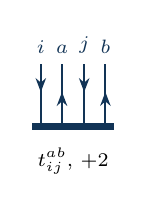
\begin{tikzpicture}[fcidiagram,baseline={(0,0)},scale=0.85]
    \draw[amp] (-0.40,0) -- (1.30,0);
    \draw[hline] (-0.22,0) -- (-0.22,1.3) node[dlab,above] {$i$};
    \draw[pline] (0.22,0) -- (0.22,1.3) node[dlab,above] {$a$};
    \draw[hline] (0.68,0) -- (0.68,1.3) node[dlab,above] {$j$};
    \draw[pline] (1.12,0) -- (1.12,1.3) node[dlab,above] {$b$};
    \node[dlab,below] at (0.45,-0.25) {$t_{ij}^{ab}$, $+2$};
\end{tikzpicture}
& 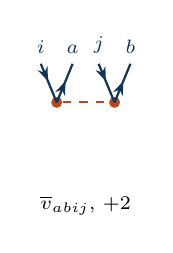
\begin{tikzpicture}[fcidiagram,baseline={(0,0)},scale=0.85]
    \node[vtx] (h0) at (-0.60,1.35) {}; \node[vtx] (h1) at (0.60,1.35) {}; \draw[vint] (h0) -- (h1);
    \draw[pline] (h0.center) -- (-0.27,2.15) node[dlab,above] {$a$};
    \draw[hline] (h0.center) -- (-0.93,2.15) node[dlab,above] {$i$};
    \draw[pline] (h1.center) -- (0.93,2.15) node[dlab,above] {$b$};
    \draw[hline] (h1.center) -- (0.27,2.15) node[dlab,above] {$j$};
    \node[dlab,below] at (0.00,-0.40) {$\overline{v}_{abij}$, $+2$};
\end{tikzpicture} & 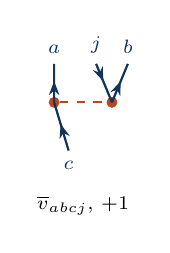
\begin{tikzpicture}[fcidiagram,baseline={(0,0)},scale=0.85]
    \node[vtx] (h0) at (-0.60,1.35) {}; \node[vtx] (h1) at (0.60,1.35) {}; \draw[vint] (h0) -- (h1);
    \draw[pline] (h0.center) -- (-0.60,2.15) node[dlab,above] {$a$};
    \draw[pline] (-0.30,0.35) node[dlab,below] {$c$} -- (h0.center);
    \draw[pline] (h1.center) -- (0.93,2.15) node[dlab,above] {$b$};
    \draw[hline] (h1.center) -- (0.27,2.15) node[dlab,above] {$j$};
    \node[dlab,below] at (0.00,-0.40) {$\overline{v}_{abcj}$, $+1$};
\end{tikzpicture} & 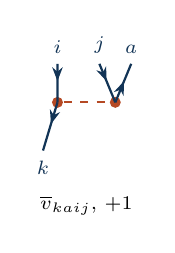
\begin{tikzpicture}[fcidiagram,baseline={(0,0)},scale=0.85]
    \node[vtx] (h0) at (-0.60,1.35) {}; \node[vtx] (h1) at (0.60,1.35) {}; \draw[vint] (h0) -- (h1);
    \draw[hline] (-0.90,0.35) node[dlab,below] {$k$} -- (h0.center);
    \draw[hline] (h0.center) -- (-0.60,2.15) node[dlab,above] {$i$};
    \draw[pline] (h1.center) -- (0.93,2.15) node[dlab,above] {$a$};
    \draw[hline] (h1.center) -- (0.27,2.15) node[dlab,above] {$j$};
    \node[dlab,below] at (0.00,-0.40) {$\overline{v}_{kaij}$, $+1$};
\end{tikzpicture}
\end{tabular}

\vspace{0.9em}
\begin{tabular}{@{}c@{\hspace{1.8em}}c@{\hspace{1.8em}}c@{\hspace{1.8em}}c@{\hspace{1.8em}}c@{\hspace{1.8em}}c@{}}
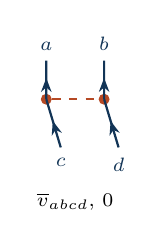
\begin{tikzpicture}[fcidiagram,baseline={(0,0)},scale=0.85]
    \node[vtx] (h0) at (-0.60,1.35) {}; \node[vtx] (h1) at (0.60,1.35) {}; \draw[vint] (h0) -- (h1);
    \draw[pline] (h0.center) -- (-0.60,2.15) node[dlab,above] {$a$};
    \draw[pline] (-0.30,0.35) node[dlab,below] {$c$} -- (h0.center);
    \draw[pline] (h1.center) -- (0.60,2.15) node[dlab,above] {$b$};
    \draw[pline] (0.90,0.35) node[dlab,below] {$d$} -- (h1.center);
    \node[dlab,below] at (0.00,-0.40) {$\overline{v}_{abcd}$, $0$};
\end{tikzpicture} & 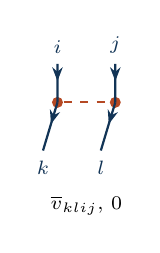
\begin{tikzpicture}[fcidiagram,baseline={(0,0)},scale=0.85]
    \node[vtx] (h0) at (-0.60,1.35) {}; \node[vtx] (h1) at (0.60,1.35) {}; \draw[vint] (h0) -- (h1);
    \draw[hline] (-0.90,0.35) node[dlab,below] {$k$} -- (h0.center);
    \draw[hline] (h0.center) -- (-0.60,2.15) node[dlab,above] {$i$};
    \draw[hline] (0.30,0.35) node[dlab,below] {$l$} -- (h1.center);
    \draw[hline] (h1.center) -- (0.60,2.15) node[dlab,above] {$j$};
    \node[dlab,below] at (0.00,-0.40) {$\overline{v}_{klij}$, $0$};
\end{tikzpicture} & 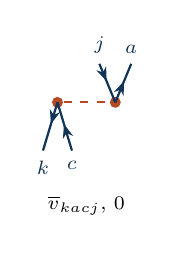
\begin{tikzpicture}[fcidiagram,baseline={(0,0)},scale=0.85]
    \node[vtx] (h0) at (-0.60,1.35) {}; \node[vtx] (h1) at (0.60,1.35) {}; \draw[vint] (h0) -- (h1);
    \draw[hline] (-0.90,0.35) node[dlab,below] {$k$} -- (h0.center);
    \draw[pline] (-0.30,0.35) node[dlab,below] {$c$} -- (h0.center);
    \draw[pline] (h1.center) -- (0.93,2.15) node[dlab,above] {$a$};
    \draw[hline] (h1.center) -- (0.27,2.15) node[dlab,above] {$j$};
    \node[dlab,below] at (0.00,-0.40) {$\overline{v}_{kacj}$, $0$};
\end{tikzpicture} & 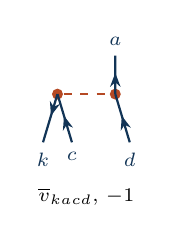
\begin{tikzpicture}[fcidiagram,baseline={(0,0)},scale=0.85]
    \node[vtx] (h0) at (-0.60,1.35) {}; \node[vtx] (h1) at (0.60,1.35) {}; \draw[vint] (h0) -- (h1);
    \draw[hline] (-0.90,0.35) node[dlab,below] {$k$} -- (h0.center);
    \draw[pline] (-0.30,0.35) node[dlab,below] {$c$} -- (h0.center);
    \draw[pline] (h1.center) -- (0.60,2.15) node[dlab,above] {$a$};
    \draw[pline] (0.90,0.35) node[dlab,below] {$d$} -- (h1.center);
    \node[dlab,below] at (0.00,-0.40) {$\overline{v}_{kacd}$, $-1$};
\end{tikzpicture} & 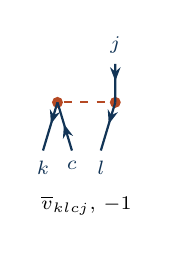
\begin{tikzpicture}[fcidiagram,baseline={(0,0)},scale=0.85]
    \node[vtx] (h0) at (-0.60,1.35) {}; \node[vtx] (h1) at (0.60,1.35) {}; \draw[vint] (h0) -- (h1);
    \draw[hline] (-0.90,0.35) node[dlab,below] {$k$} -- (h0.center);
    \draw[pline] (-0.30,0.35) node[dlab,below] {$c$} -- (h0.center);
    \draw[hline] (0.30,0.35) node[dlab,below] {$l$} -- (h1.center);
    \draw[hline] (h1.center) -- (0.60,2.15) node[dlab,above] {$j$};
    \node[dlab,below] at (0.00,-0.40) {$\overline{v}_{klcj}$, $-1$};
\end{tikzpicture} & 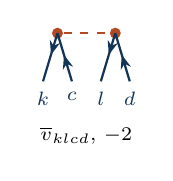
\begin{tikzpicture}[fcidiagram,baseline={(0,0)},scale=0.85]
    \node[vtx] (h0) at (-0.60,1.35) {}; \node[vtx] (h1) at (0.60,1.35) {}; \draw[vint] (h0) -- (h1);
    \draw[hline] (-0.90,0.35) node[dlab,below] {$k$} -- (h0.center);
    \draw[pline] (-0.30,0.35) node[dlab,below] {$c$} -- (h0.center);
    \draw[hline] (0.30,0.35) node[dlab,below] {$l$} -- (h1.center);
    \draw[pline] (0.90,0.35) node[dlab,below] {$d$} -- (h1.center);
    \node[dlab,below] at (0.00,-0.40) {$\overline{v}_{klcd}$, $-2$};
\end{tikzpicture}
\end{tabular}
\end{center}
\vspace{0.3em}
\footnotesize Top row: the four fragments of $F_N$ (crosses), the cluster operator $T_2$ (bar), and the three fragments of $V_N$ that excite. Bottom row: the six fragments of $V_N$ of level $0$, $-1$ and $-2$. Each fragment carries its matrix element and its \emph{excitation level}: the number of particle-hole pairs it creates (lines leaving upwards minus lines entering from below, divided by two). Interaction: $\as{\text{left out}}{\text{right out}}{\text{left in}}{\text{right in}}$, with ``out'' the line leaving a vertex upwards and ``in'' the line entering from below; cross: $f_{\text{out},\text{in}}$.
\end{frame}

\begin{frame}[shrink=3]{Bookkeeping by excitation level}
The projection fixes the level at the top of the diagram: $0$ for the energy, $+2$ for the doubles equation. Each $T_2$ contributes $+2$. The fragment of $H_N$ must supply the difference.
\begin{center}
\renewcommand{\arraystretch}{1.3}
\begin{tabular}{lccl}
\toprule
projection & bars & level of the $H_N$ fragment & fragments that fit\\
\midrule
energy ($0$) & $T_2$ & $-2$ & $\as klcd$\\
\midrule
doubles ($+2$) & none & $+2$ & $\as abij$\\
doubles ($+2$) & $T_2$ & $0$ & $f_{bc}$, $f_{kj}$, $\as abcd$, $\as klij$, $\as kbcj$\\
doubles ($+2$) & $T_2T_2$ & $-2$ & $\as klcd$\\
\bottomrule
\end{tabular}
\end{center}
\begin{itemize}
\item This is yesterday's operator counting in one table: ten diagrams at most, before anything is drawn. (The level $-2$ fragment can attach to two bars in four inequivalent ways.)
\item The fragments $f_{ai}$, $f_{ia}$, $\as abcj$, $\as kaij$, $\as kacd$, $\as klcj$ change the level by an odd number. With $T_2$ alone they can never give a double: they belong to the singles, next week.
\end{itemize}
\end{frame}

\begin{frame}[shrink=7]{Drawing and reading: the rules}
\small
\begin{block}{Drawing}
Attach one fragment of $H_N$ to zero, one or two bars in every distinct way that leaves $i,j,a,b$ open at the top. Every bar must be attached to $H_N$ by at least one line. No line runs between two bars.
\end{block}
\begin{block}{Reading (chapter 9, section 9.15, without the denominators)}
\begin{enumerate}
\item Label every line; external lines carry the labels of $\bra{\Phi_{ij}^{ab}}$. Sum over internal labels.
\item Cross: $f_{\text{out},\text{in}}$. Interaction: $\as{\text{left out}}{\text{right out}}{\text{left in}}{\text{right in}}$. Bar: $t_{\text{holes}}^{\text{particles}}$, vertices left to right.
\item Sign $(-1)^{h+l}$: $h$ = number of hole lines (internal and external), $l$ = number of loops. External lines are closed through the bra: $i$ with $a$, $j$ with $b$.
\item $\tfrac12$ for each pair of equivalent lines (same kind, same two operators, same direction) and for each pair of equivalent vertices (two bars attached to $H_N$ in the same way).
\item $P(ab)$ if the external particle lines leave from different operators, $P(ij)$ likewise for the external hole lines.
\end{enumerate}
\end{block}
These are theorems about Wick contractions (week 45), not conventions. Every reading below can be -- and has been, yesterday -- checked by contracting operators.
\end{frame}

\begin{frame}{The energy and the driving term}
\small
\begin{columns}[T]
\column{0.5\textwidth}
\centering
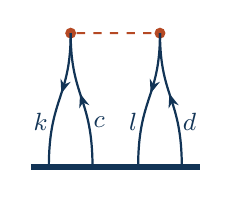
\begin{tikzpicture}[fcidiagram,dlab/.style={font=\small},scale=1.75]
    \draw[amp] (-0.40,0) -- (1.30,0);
    \node[vtx] (h0) at (0.00,1.35) {}; \node[vtx] (h1) at (0.90,1.35) {}; \draw[vint] (h0) -- (h1);
    \draw[hline] (-0.22,0) .. controls (-0.22,0.7) and (0.00,0.7) .. node[dlab,left,pos=0.28,inner sep=1.5pt] {$k$} (h0.center);
    \draw[pline] (0.22,0) .. controls (0.22,0.7) and (0.00,0.7) .. node[dlab,right,pos=0.28,inner sep=1.5pt] {$c$} (h0.center);
    \draw[hline] (0.68,0) .. controls (0.68,0.7) and (0.90,0.7) .. node[dlab,left,pos=0.28,inner sep=1.5pt] {$l$} (h1.center);
    \draw[pline] (1.12,0) .. controls (1.12,0.7) and (0.90,0.7) .. node[dlab,right,pos=0.28,inner sep=1.5pt] {$d$} (h1.center);
\end{tikzpicture}

\vspace{0.6em}
\raggedright
\textbf{Energy.} $\as klcd$ closes the bar completely.
\begin{itemize}
\item hole lines $k,l$: $h=2$; loops $(k,c)$, $(l,d)$: $l=2$; sign $+$
\item $c,d$ are equivalent, $k,l$ are equivalent: $\tfrac12\cdot\tfrac12$
\end{itemize}
\[
 \Delta E=+\frac14\sum_{klcd}\as klcd\,t_{kl}^{cd}
\]
\column{0.5\textwidth}
\centering
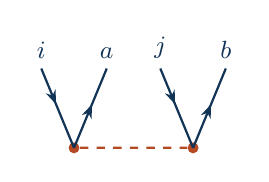
\begin{tikzpicture}[fcidiagram,dlab/.style={font=\small},scale=1.75]
    \node[vtx] (h0) at (-0.60,1.35) {}; \node[vtx] (h1) at (0.60,1.35) {}; \draw[vint] (h0) -- (h1);
    \draw[pline] (h0.center) -- (-0.27,2.15) node[dlab,above] {$a$};
    \draw[hline] (h0.center) -- (-0.93,2.15) node[dlab,above] {$i$};
    \draw[pline] (h1.center) -- (0.93,2.15) node[dlab,above] {$b$};
    \draw[hline] (h1.center) -- (0.27,2.15) node[dlab,above] {$j$};
\end{tikzpicture}

\vspace{0.6em}
\raggedright
\textbf{Driving term.} The level $+2$ fragment alone.
\begin{itemize}
\item $h=2$ ($i,j$); closed through the bra, $(i,a)$ and $(j,b)$ are two loops: sign $+$
\item no internal lines: nothing to sum, no $\tfrac12$
\item $a,b$ leave from the same operator, $i,j$ too: no $P$
\end{itemize}
\[
 +\as abij
\]
\end{columns}
\vspace{0.4em}
Compare with yesterday: four equal patterns times $\tfrac1{16}$, and four times $\tfrac14$.
\end{frame}

\begin{frame}[shrink=1]{The two Fock diagrams}
\small
\begin{columns}[T]
\column{0.5\textwidth}
\centering
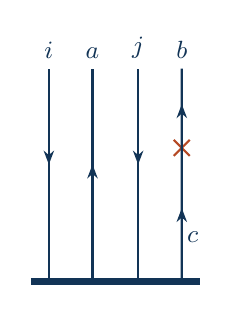
\begin{tikzpicture}[fcidiagram,dlab/.style={font=\small},scale=1.75]
    \draw[amp] (-0.40,0) -- (1.30,0);
    \node[fvtx] (h0) at (1.12,1.35) {};
    \draw[pline] (h0.center) -- (1.12,2.15) node[dlab,above] {$b$};
    \draw[pline] (1.12,0) .. controls (1.12,0.7) and (1.12,0.7) .. node[dlab,right,pos=0.28,inner sep=1.5pt] {$c$} (h0.center);
    \draw[hline] (-0.22,0) -- (-0.22,2.15) node[dlab,above] {$i$};
    \draw[pline] (0.22,0) -- (0.22,2.15) node[dlab,above] {$a$};
    \draw[hline] (0.68,0) -- (0.68,2.15) node[dlab,above] {$j$};
\end{tikzpicture}

\vspace{0.6em}
\raggedright
\textbf{Cross on a particle line.} The line $c$ leaves the bar, is scattered by $f_{bc}$ and leaves as $b$.
\begin{itemize}
\item $h=2$ ($i,j$); loops $(i,a)$ and $(j\!\to\!c\!\to\!b)$: $l=2$; sign $+$
\item no equivalent lines
\item $a$ leaves from the bar, $b$ from the cross: $P(ab)$
\end{itemize}
\[
 +P(ab)\sum_cf_{bc}\,t_{ij}^{ac}
\]
\column{0.5\textwidth}
\centering
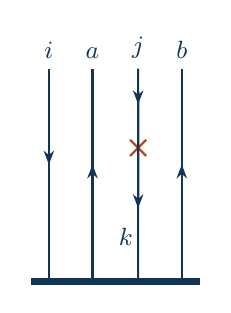
\begin{tikzpicture}[fcidiagram,dlab/.style={font=\small},scale=1.75]
    \draw[amp] (-0.40,0) -- (1.30,0);
    \node[fvtx] (h0) at (0.68,1.35) {};
    \draw[hline] (0.68,0) .. controls (0.68,0.7) and (0.68,0.7) .. node[dlab,left,pos=0.28,inner sep=1.5pt] {$k$} (h0.center);
    \draw[hline] (h0.center) -- (0.68,2.15) node[dlab,above] {$j$};
    \draw[hline] (-0.22,0) -- (-0.22,2.15) node[dlab,above] {$i$};
    \draw[pline] (0.22,0) -- (0.22,2.15) node[dlab,above] {$a$};
    \draw[pline] (1.12,0) -- (1.12,2.15) node[dlab,above] {$b$};
\end{tikzpicture}

\vspace{0.6em}
\raggedright
\textbf{Cross on a hole line.} The hole $k$ of the bar becomes the hole $j$.
\begin{itemize}
\item $h=3$ ($i,j,k$); loops $(i,a)$ and $(j\!\to\!k\!\to\!b)$: $l=2$; sign $-$
\item no equivalent lines
\item $i$ leaves from the bar, $j$ from the cross: $P(ij)$
\end{itemize}
\[
 -P(ij)\sum_kf_{kj}\,t_{ik}^{ab}
\]
\end{columns}
\vspace{0.4em}
The extra hole line is yesterday's $\ann m$ pulled through three operators.
\end{frame}

\begin{frame}[shrink=13]{The two ladder diagrams}
\small
\begin{columns}[T]
\column{0.5\textwidth}
\centering
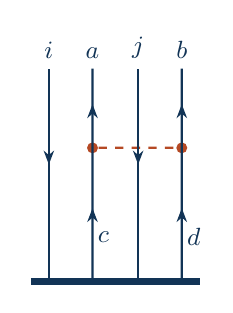
\begin{tikzpicture}[fcidiagram,dlab/.style={font=\small},scale=1.75]
    \draw[amp] (-0.40,0) -- (1.30,0);
    \node[vtx] (h0) at (0.22,1.35) {}; \node[vtx] (h1) at (1.12,1.35) {}; \draw[vint] (h0) -- (h1);
    \draw[pline] (h0.center) -- (0.22,2.15) node[dlab,above] {$a$};
    \draw[pline] (0.22,0) .. controls (0.22,0.7) and (0.22,0.7) .. node[dlab,right,pos=0.28,inner sep=1.5pt] {$c$} (h0.center);
    \draw[pline] (h1.center) -- (1.12,2.15) node[dlab,above] {$b$};
    \draw[pline] (1.12,0) .. controls (1.12,0.7) and (1.12,0.7) .. node[dlab,right,pos=0.28,inner sep=1.5pt] {$d$} (h1.center);
    \draw[hline] (-0.22,0) -- (-0.22,2.15) node[dlab,above] {$i$};
    \draw[hline] (0.68,0) -- (0.68,2.15) node[dlab,above] {$j$};
\end{tikzpicture}

\vspace{0.6em}
\raggedright
\textbf{Particle-particle ladder.} Both particle lines of the bar enter $\as abcd$.
\begin{itemize}
\item $h=2$, $l=2$: sign $+$
\item $c,d$ equivalent: $\tfrac12$
\item $a,b$ both from the interaction, $i,j$ both from the bar: no $P$
\end{itemize}
\[
 +\frac12\sum_{cd}\as abcd\,t_{ij}^{cd}
\]
\column{0.5\textwidth}
\centering
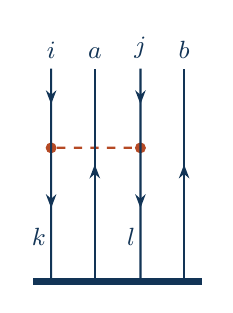
\begin{tikzpicture}[fcidiagram,dlab/.style={font=\small},scale=1.75]
    \draw[amp] (-0.40,0) -- (1.30,0);
    \node[vtx] (h0) at (-0.22,1.35) {}; \node[vtx] (h1) at (0.68,1.35) {}; \draw[vint] (h0) -- (h1);
    \draw[hline] (-0.22,0) .. controls (-0.22,0.7) and (-0.22,0.7) .. node[dlab,left,pos=0.28,inner sep=1.5pt] {$k$} (h0.center);
    \draw[hline] (h0.center) -- (-0.22,2.15) node[dlab,above] {$i$};
    \draw[hline] (0.68,0) .. controls (0.68,0.7) and (0.68,0.7) .. node[dlab,left,pos=0.28,inner sep=1.5pt] {$l$} (h1.center);
    \draw[hline] (h1.center) -- (0.68,2.15) node[dlab,above] {$j$};
    \draw[pline] (0.22,0) -- (0.22,2.15) node[dlab,above] {$a$};
    \draw[pline] (1.12,0) -- (1.12,2.15) node[dlab,above] {$b$};
\end{tikzpicture}

\vspace{0.6em}
\raggedright
\textbf{Hole-hole ladder.} Both hole lines of the bar enter $\as klij$.
\begin{itemize}
\item $h=4$ ($i,j,k,l$), $l=2$: sign $+$
\item $k,l$ equivalent: $\tfrac12$
\item no $P$
\end{itemize}
\[
 +\frac12\sum_{kl}\as klij\,t_{kl}^{ab}
\]
\end{columns}
\vspace{0.4em}
Replace the bar by its first-order value $\as cdij/D_{ij}^{cd}$ and close with $\as ijab$: the particle-particle and hole-hole ladder diagrams of third-order perturbation theory (week 45).
\end{frame}

\begin{frame}[shrink=1]{The ring diagram}
\small
\begin{columns}[T]
\column{0.42\textwidth}
\centering
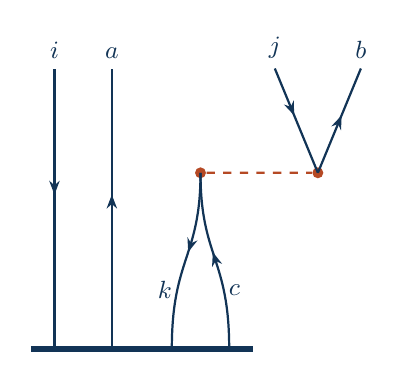
\begin{tikzpicture}[fcidiagram,dlab/.style={font=\small},scale=2.3]
    \draw[amp] (-0.40,0) -- (1.30,0);
    \node[vtx] (h0) at (0.90,1.35) {}; \node[vtx] (h1) at (1.80,1.35) {}; \draw[vint] (h0) -- (h1);
    \draw[hline] (0.68,0) .. controls (0.68,0.7) and (0.90,0.7) .. node[dlab,left,pos=0.28,inner sep=1.5pt] {$k$} (h0.center);
    \draw[pline] (1.12,0) .. controls (1.12,0.7) and (0.90,0.7) .. node[dlab,right,pos=0.28,inner sep=1.5pt] {$c$} (h0.center);
    \draw[pline] (h1.center) -- (2.13,2.15) node[dlab,above] {$b$};
    \draw[hline] (h1.center) -- (1.47,2.15) node[dlab,above] {$j$};
    \draw[hline] (-0.22,0) -- (-0.22,2.15) node[dlab,above] {$i$};
    \draw[pline] (0.22,0) -- (0.22,2.15) node[dlab,above] {$a$};
\end{tikzpicture}
\column{0.58\textwidth}
\textbf{One particle and one hole line} of the bar enter the same vertex of $\as kbcj$; the other vertex emits the new pair $(b,j)$.
\begin{itemize}
\item hole lines $i,j,k$: $h=3$
\item loops: $(i,a)$ through the bra; $(k,c)$ between the bar and the left vertex; $(j,b)$ through the bra: $l=3$
\item sign $(-1)^{3+3}=+$
\item no equivalent lines: $k$ and $c$ are of different kind
\item $a$ from the bar and $b$ from the interaction: $P(ab)$; $i$ from the bar and $j$ from the interaction: $P(ij)$
\end{itemize}
\[
 +P(ij)P(ab)\sum_{kc}\as kbcj\,t_{ik}^{ac}
\]
\end{columns}
\vspace{0.5em}
Yesterday this term needed sixteen patterns, a relabelling and two sign flips. Here the closed loop $(k,c)$ -- the ``ring'' -- supplies the sign that compensates the third hole line. With the bar at first order and closed from above: the third-order particle-hole diagram of week 45, and the first link of the RPA chain.
\end{frame}

\begin{frame}{Pause to think \#5}
\thinkq{4}{\normalsize
\begin{columns}[c]
\column{0.36\textwidth}
\centering
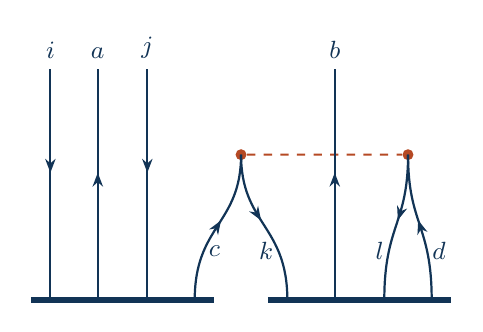
\begin{tikzpicture}[fcidiagram,dlab/.style={font=\small},scale=1.9]
    \draw[amp] (-0.40,0) -- (1.30,0);
    \draw[amp] (1.80,0) -- (3.50,0);
    \node[vtx] (h0) at (1.55,1.35) {}; \node[vtx] (h1) at (3.10,1.35) {}; \draw[vint] (h0) -- (h1);
    \draw[hline] (1.98,0) .. controls (1.98,0.7) and (1.55,0.7) .. node[dlab,left,pos=0.28,inner sep=1.5pt] {$k$} (h0.center);
    \draw[pline] (1.12,0) .. controls (1.12,0.7) and (1.55,0.7) .. node[dlab,right,pos=0.28,inner sep=1.5pt] {$c$} (h0.center);
    \draw[hline] (2.88,0) .. controls (2.88,0.7) and (3.10,0.7) .. node[dlab,left,pos=0.28,inner sep=1.5pt] {$l$} (h1.center);
    \draw[pline] (3.32,0) .. controls (3.32,0.7) and (3.10,0.7) .. node[dlab,right,pos=0.28,inner sep=1.5pt] {$d$} (h1.center);
    \draw[hline] (-0.22,0) -- (-0.22,2.15) node[dlab,above] {$i$};
    \draw[pline] (0.22,0) -- (0.22,2.15) node[dlab,above] {$a$};
    \draw[hline] (0.68,0) -- (0.68,2.15) node[dlab,above] {$j$};
    \draw[pline] (2.42,0) -- (2.42,2.15) node[dlab,above] {$b$};
\end{tikzpicture}
\column{0.64\textwidth}
One of the four diagrams with two bars.
\begin{enumerate}
\item Which bar takes one line of the interaction, which takes three?
\item Read it: matrix element, amplitudes, sign $(-1)^{h+l}$, factors $\tfrac12$, permutations.
\item Which of yesterday's four terms $Q_a,\dots,Q_d$ is it, and which dressed vertex $\chi$ do you see in the picture?
\end{enumerate}
\end{columns}}
\end{frame}

\begin{frame}[shrink=1]{Answer to pause \#5}
\thinka{%
\begin{enumerate}
\item The left bar, $t_{ij}^{ac}$, gives only the particle line $c$. The right bar, $t_{kl}^{bd}$, gives $k$, $l$ and $d$ and keeps only $b$.
\item $\as klcd\,t_{ij}^{ac}\,t_{kl}^{bd}$. Hole lines $i,j,k,l$: $h=4$. Loops: $(i,a)$; $(l,d)$ between the right bar and the right vertex; and $j\to c\to k\to b$ through the bra: $l=3$. Sign $-$. The lines $k$ and $l$ are equivalent (two hole lines from the same bar to the same interaction): $\tfrac12$. $a$ and $b$ leave from different bars: $P(ab)$; $i,j$ from the same bar: no $P(ij)$.
\[
 -\tfrac12P(ab)\sum_{klcd}\as klcd\,t_{ij}^{ac}\,t_{kl}^{bd}
\]
\item $Q_c$. Cover the left bar: what remains -- interaction plus right bar, with one particle line $c$ entering and one, $b$, leaving -- is the dressed particle Fock vertex $\chi_{cb}=-\tfrac12\as klcd\,t_{kl}^{bd}$. The whole diagram is the particle Fock diagram with $f_{bc}\to\chi_{cb}$.
\end{enumerate}}
\end{frame}

\begin{frame}[shrink=10]{Two bars: $Q_a$ and $Q_b$}
\small
\begin{columns}[T]
\column{0.5\textwidth}
\centering
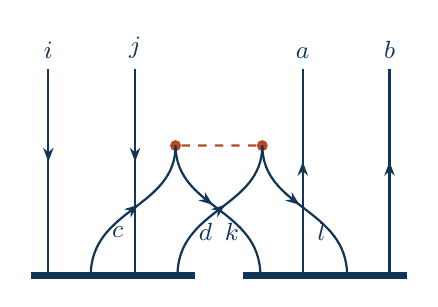
\begin{tikzpicture}[fcidiagram,dlab/.style={font=\small},scale=1.7]
    \draw[amp] (-0.40,0) -- (1.30,0);
    \draw[amp] (1.80,0) -- (3.50,0);
    \node[vtx] (h0) at (1.10,1.35) {}; \node[vtx] (h1) at (2.00,1.35) {}; \draw[vint] (h0) -- (h1);
    \draw[hline] (1.98,0) .. controls (1.98,0.7) and (1.10,0.7) .. node[dlab,left,pos=0.28,inner sep=1.5pt] {$k$} (h0.center);
    \draw[pline] (0.22,0) .. controls (0.22,0.7) and (1.10,0.7) .. node[dlab,right,pos=0.28,inner sep=1.5pt] {$c$} (h0.center);
    \draw[hline] (2.88,0) .. controls (2.88,0.7) and (2.00,0.7) .. node[dlab,left,pos=0.28,inner sep=1.5pt] {$l$} (h1.center);
    \draw[pline] (1.12,0) .. controls (1.12,0.7) and (2.00,0.7) .. node[dlab,right,pos=0.28,inner sep=1.5pt] {$d$} (h1.center);
    \draw[hline] (-0.22,0) -- (-0.22,2.15) node[dlab,above] {$i$};
    \draw[hline] (0.68,0) -- (0.68,2.15) node[dlab,above] {$j$};
    \draw[pline] (2.42,0) -- (2.42,2.15) node[dlab,above] {$a$};
    \draw[pline] (3.32,0) -- (3.32,2.15) node[dlab,above] {$b$};
\end{tikzpicture}

\vspace{0.5em}
\raggedright
$Q_a$: one bar gives both particle lines, the other both hole lines.
\begin{itemize}
\item $h=4$; loops $(i\!\to\!c\!\to\!k\!\to\!a)$ and $(j\!\to\!d\!\to\!l\!\to\!b)$: $l=2$; sign $+$
\item $(c,d)$ equivalent and $(k,l)$ equivalent: $\tfrac14$
\item $i,j$ from one bar, $a,b$ from the other: no $P$
\end{itemize}
\[
 +\frac14\as klcd\,t_{ij}^{cd}\,t_{kl}^{ab}
\]
\column{0.5\textwidth}
\centering
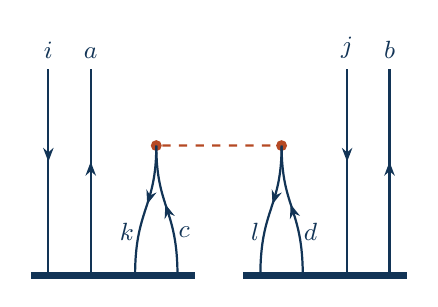
\begin{tikzpicture}[fcidiagram,dlab/.style={font=\small},scale=1.7]
    \draw[amp] (-0.40,0) -- (1.30,0);
    \draw[amp] (1.80,0) -- (3.50,0);
    \node[vtx] (h0) at (0.90,1.35) {}; \node[vtx] (h1) at (2.20,1.35) {}; \draw[vint] (h0) -- (h1);
    \draw[hline] (0.68,0) .. controls (0.68,0.7) and (0.90,0.7) .. node[dlab,left,pos=0.28,inner sep=1.5pt] {$k$} (h0.center);
    \draw[pline] (1.12,0) .. controls (1.12,0.7) and (0.90,0.7) .. node[dlab,right,pos=0.28,inner sep=1.5pt] {$c$} (h0.center);
    \draw[hline] (1.98,0) .. controls (1.98,0.7) and (2.20,0.7) .. node[dlab,left,pos=0.28,inner sep=1.5pt] {$l$} (h1.center);
    \draw[pline] (2.42,0) .. controls (2.42,0.7) and (2.20,0.7) .. node[dlab,right,pos=0.28,inner sep=1.5pt] {$d$} (h1.center);
    \draw[hline] (-0.22,0) -- (-0.22,2.15) node[dlab,above] {$i$};
    \draw[pline] (0.22,0) -- (0.22,2.15) node[dlab,above] {$a$};
    \draw[hline] (2.88,0) -- (2.88,2.15) node[dlab,above] {$j$};
    \draw[pline] (3.32,0) -- (3.32,2.15) node[dlab,above] {$b$};
\end{tikzpicture}

\vspace{0.5em}
\raggedright
$Q_b$: each bar gives one particle-hole pair -- a ring on each side.
\begin{itemize}
\item $h=4$; loops $(i,a)$, $(k,c)$, $(l,d)$, $(j,b)$: $l=4$; sign $+$
\item no equivalent lines, but the two bars are equivalent vertices: $\tfrac12$
\item $i,j$ from different bars, $a,b$ too: $P(ij)P(ab)$
\end{itemize}
\[
 +\frac12P(ij)P(ab)\as klcd\,t_{ik}^{ac}\,t_{jl}^{bd}
\]
\end{columns}
\vspace{0.3em}
$Q_a$ is the hole-hole ladder with $\as klij\to\chi_{klij}$; $Q_b$ is the ring with $\as kbcj\to\chi_{bkcj}$.
\end{frame}

\begin{frame}[shrink=10]{Two bars: $Q_c$ and $Q_d$}
\small
\begin{columns}[T]
\column{0.5\textwidth}
\centering
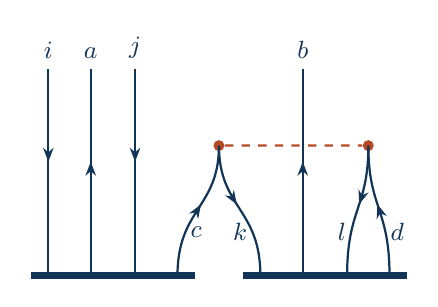
\begin{tikzpicture}[fcidiagram,dlab/.style={font=\small},scale=1.7]
    \draw[amp] (-0.40,0) -- (1.30,0);
    \draw[amp] (1.80,0) -- (3.50,0);
    \node[vtx] (h0) at (1.55,1.35) {}; \node[vtx] (h1) at (3.10,1.35) {}; \draw[vint] (h0) -- (h1);
    \draw[hline] (1.98,0) .. controls (1.98,0.7) and (1.55,0.7) .. node[dlab,left,pos=0.28,inner sep=1.5pt] {$k$} (h0.center);
    \draw[pline] (1.12,0) .. controls (1.12,0.7) and (1.55,0.7) .. node[dlab,right,pos=0.28,inner sep=1.5pt] {$c$} (h0.center);
    \draw[hline] (2.88,0) .. controls (2.88,0.7) and (3.10,0.7) .. node[dlab,left,pos=0.28,inner sep=1.5pt] {$l$} (h1.center);
    \draw[pline] (3.32,0) .. controls (3.32,0.7) and (3.10,0.7) .. node[dlab,right,pos=0.28,inner sep=1.5pt] {$d$} (h1.center);
    \draw[hline] (-0.22,0) -- (-0.22,2.15) node[dlab,above] {$i$};
    \draw[pline] (0.22,0) -- (0.22,2.15) node[dlab,above] {$a$};
    \draw[hline] (0.68,0) -- (0.68,2.15) node[dlab,above] {$j$};
    \draw[pline] (2.42,0) -- (2.42,2.15) node[dlab,above] {$b$};
\end{tikzpicture}

\vspace{0.5em}
\raggedright
$Q_c$: three lines $(k,l,d)$ from one bar, one particle line from the other.
\begin{itemize}
\item $h=4$, $l=3$: sign $-$
\item $(k,l)$ equivalent: $\tfrac12$
\item $a,b$ from different bars: $P(ab)$
\end{itemize}
\[
 -\frac12P(ab)\as klcd\,t_{ij}^{ac}\,t_{kl}^{bd}
\]
\column{0.5\textwidth}
\centering
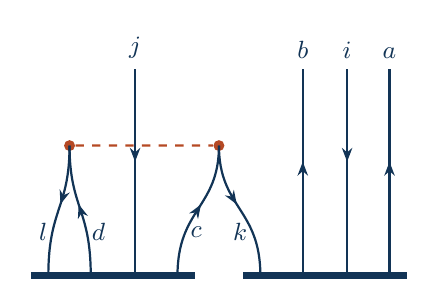
\begin{tikzpicture}[fcidiagram,dlab/.style={font=\small},scale=1.7]
    \draw[amp] (-0.40,0) -- (1.30,0);
    \draw[amp] (1.80,0) -- (3.50,0);
    \node[vtx] (h0) at (0.00,1.35) {}; \node[vtx] (h1) at (1.55,1.35) {}; \draw[vint] (h0) -- (h1);
    \draw[hline] (-0.22,0) .. controls (-0.22,0.7) and (0.00,0.7) .. node[dlab,left,pos=0.28,inner sep=1.5pt] {$l$} (h0.center);
    \draw[pline] (0.22,0) .. controls (0.22,0.7) and (0.00,0.7) .. node[dlab,right,pos=0.28,inner sep=1.5pt] {$d$} (h0.center);
    \draw[hline] (1.98,0) .. controls (1.98,0.7) and (1.55,0.7) .. node[dlab,left,pos=0.28,inner sep=1.5pt] {$k$} (h1.center);
    \draw[pline] (1.12,0) .. controls (1.12,0.7) and (1.55,0.7) .. node[dlab,right,pos=0.28,inner sep=1.5pt] {$c$} (h1.center);
    \draw[hline] (0.68,0) -- (0.68,2.15) node[dlab,above] {$j$};
    \draw[pline] (2.42,0) -- (2.42,2.15) node[dlab,above] {$b$};
    \draw[hline] (2.88,0) -- (2.88,2.15) node[dlab,above] {$i$};
    \draw[pline] (3.32,0) -- (3.32,2.15) node[dlab,above] {$a$};
\end{tikzpicture}

\vspace{0.5em}
\raggedright
$Q_d$: three lines $(l,c,d)$ from one bar, one hole line from the other.
\begin{itemize}
\item $h=4$; loops $(l,d)$, $(i,a)$ and $(j\!\to\!c\!\to\!k\!\to\!b)$: $l=3$; sign $-$
\item $(c,d)$ equivalent: $\tfrac12$
\item $i,j$ from different bars: $P(ij)$
\end{itemize}
\[
 -\frac12P(ij)\as klcd\,t_{ik}^{ab}\,t_{jl}^{cd}
\]
\end{columns}
\vspace{0.3em}
The Fock diagrams with $f_{bc}\to\chi_{cb}$ and $f_{kj}\to\chi_{kj}$: the interaction and one bar form a ``self-energy insertion'' on a line of the other bar.
\end{frame}

\begin{frame}{Two pictures that are not drawn}
\small
\begin{columns}[T]
\column{0.5\textwidth}
\centering
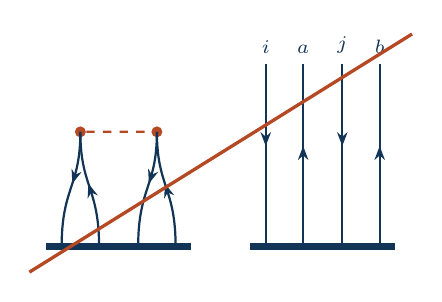
\begin{tikzpicture}[fcidiagram,scale=1.5]
    \draw[amp] (-0.40,0) -- (1.30,0);
    \draw[amp] (2.00,0) -- (3.70,0);
    \node[vtx] (h0) at (0.00,1.35) {}; \node[vtx] (h1) at (0.90,1.35) {}; \draw[vint] (h0) -- (h1);
    \draw[hline] (-0.22,0) .. controls (-0.22,0.7) and (0.00,0.7) .. (h0.center);
    \draw[pline] (0.22,0) .. controls (0.22,0.7) and (0.00,0.7) .. (h0.center);
    \draw[hline] (0.68,0) .. controls (0.68,0.7) and (0.90,0.7) .. (h1.center);
    \draw[pline] (1.12,0) .. controls (1.12,0.7) and (0.90,0.7) .. (h1.center);
    \draw[hline] (2.18,0) -- (2.18,2.15) node[dlab,above] {$i$};
    \draw[pline] (2.62,0) -- (2.62,2.15) node[dlab,above] {$a$};
    \draw[hline] (3.08,0) -- (3.08,2.15) node[dlab,above] {$j$};
    \draw[pline] (3.52,0) -- (3.52,2.15) node[dlab,above] {$b$};
    \draw[warm,line width=1.2pt] (-0.6,-0.3) -- (3.9,2.5);
\end{tikzpicture}

\vspace{0.6em}
\raggedright
\textbf{A bar attached to nothing.} This is $\Delta E\times t_{ij}^{ab}$: yesterday's fifth distribution. It is \emph{unlinked} -- a closed piece beside an open one -- and it is the term that $-T_2H_NT_2$ cancels. The subscript $c$ forbids it.
\column{0.5\textwidth}
\centering
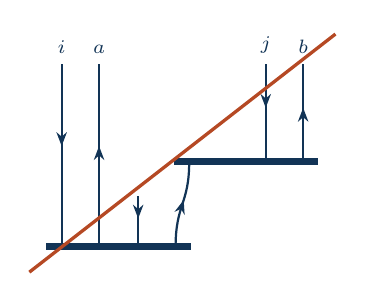
\begin{tikzpicture}[fcidiagram,scale=1.5]
    \draw[amp] (-0.40,0) -- (1.30,0);
    \draw[amp] (1.10,1.0) -- (2.80,1.0);
    \draw[hline] (-0.22,0) -- (-0.22,2.15) node[dlab,above] {$i$};
    \draw[pline] (0.22,0) -- (0.22,2.15) node[dlab,above] {$a$};
    \draw[hline] (0.68,0) -- (0.68,0.6);
    \draw[pline] (1.12,0) .. controls (1.12,0.5) and (1.28,0.5) .. (1.28,1.0);
    \draw[hline] (2.18,1.0) -- (2.18,2.15) node[dlab,above] {$j$};
    \draw[pline] (2.62,1.0) -- (2.62,2.15) node[dlab,above] {$b$};
    \draw[warm,line width=1.2pt] (-0.6,-0.3) -- (3.0,2.5);
\end{tikzpicture}

\vspace{0.6em}
\raggedright
\textbf{A line between two bars.} Both ends of such a line would be quasi-particle creation operators ($\cre a$ or $\ann i$): the contraction vanishes. Amplitudes never talk to each other directly, only through $H_N$. This is why the series stops, and why all bars can be drawn at the same height.
\end{columns}
\vspace{0.6em}
Unitary coupled cluster, $e^{T-T^\dagger}$, has de-excitation operators in the exponent: lines between cluster operators exist, and the series does not terminate (chapter 10, section 10.15; FYS5419 in the spring).
\end{frame}

\begin{frame}[shrink=13]{The CCD equation in pictures}
\small
\begin{center}
\begin{tabular}{@{}c@{\hspace{1.2em}}c@{\hspace{1.2em}}c@{\hspace{1.2em}}c@{\hspace{1.2em}}c@{\hspace{1.2em}}c@{}}
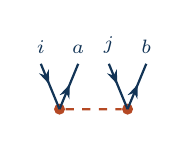
\begin{tikzpicture}[fcidiagram,scale=1.0]
    \node[vtx] (h0) at (-0.60,1.35) {}; \node[vtx] (h1) at (0.60,1.35) {}; \draw[vint] (h0) -- (h1);
    \draw[pline] (h0.center) -- (-0.27,2.15) node[dlab,above] {$a$};
    \draw[hline] (h0.center) -- (-0.93,2.15) node[dlab,above] {$i$};
    \draw[pline] (h1.center) -- (0.93,2.15) node[dlab,above] {$b$};
    \draw[hline] (h1.center) -- (0.27,2.15) node[dlab,above] {$j$};
\end{tikzpicture} & 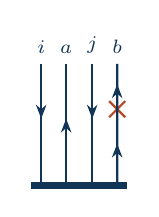
\begin{tikzpicture}[fcidiagram,scale=1.0]
    \draw[amp] (-0.40,0) -- (1.30,0);
    \node[fvtx] (h0) at (1.12,1.35) {};
    \draw[pline] (h0.center) -- (1.12,2.15) node[dlab,above] {$b$};
    \draw[pline] (1.12,0) .. controls (1.12,0.7) and (1.12,0.7) .. (h0.center);
    \draw[hline] (-0.22,0) -- (-0.22,2.15) node[dlab,above] {$i$};
    \draw[pline] (0.22,0) -- (0.22,2.15) node[dlab,above] {$a$};
    \draw[hline] (0.68,0) -- (0.68,2.15) node[dlab,above] {$j$};
\end{tikzpicture} & 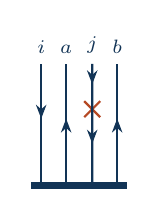
\begin{tikzpicture}[fcidiagram,scale=1.0]
    \draw[amp] (-0.40,0) -- (1.30,0);
    \node[fvtx] (h0) at (0.68,1.35) {};
    \draw[hline] (0.68,0) .. controls (0.68,0.7) and (0.68,0.7) .. (h0.center);
    \draw[hline] (h0.center) -- (0.68,2.15) node[dlab,above] {$j$};
    \draw[hline] (-0.22,0) -- (-0.22,2.15) node[dlab,above] {$i$};
    \draw[pline] (0.22,0) -- (0.22,2.15) node[dlab,above] {$a$};
    \draw[pline] (1.12,0) -- (1.12,2.15) node[dlab,above] {$b$};
\end{tikzpicture} & 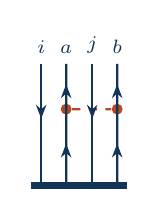
\begin{tikzpicture}[fcidiagram,scale=1.0]
    \draw[amp] (-0.40,0) -- (1.30,0);
    \node[vtx] (h0) at (0.22,1.35) {}; \node[vtx] (h1) at (1.12,1.35) {}; \draw[vint] (h0) -- (h1);
    \draw[pline] (h0.center) -- (0.22,2.15) node[dlab,above] {$a$};
    \draw[pline] (0.22,0) .. controls (0.22,0.7) and (0.22,0.7) .. (h0.center);
    \draw[pline] (h1.center) -- (1.12,2.15) node[dlab,above] {$b$};
    \draw[pline] (1.12,0) .. controls (1.12,0.7) and (1.12,0.7) .. (h1.center);
    \draw[hline] (-0.22,0) -- (-0.22,2.15) node[dlab,above] {$i$};
    \draw[hline] (0.68,0) -- (0.68,2.15) node[dlab,above] {$j$};
\end{tikzpicture} & 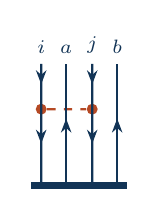
\begin{tikzpicture}[fcidiagram,scale=1.0]
    \draw[amp] (-0.40,0) -- (1.30,0);
    \node[vtx] (h0) at (-0.22,1.35) {}; \node[vtx] (h1) at (0.68,1.35) {}; \draw[vint] (h0) -- (h1);
    \draw[hline] (-0.22,0) .. controls (-0.22,0.7) and (-0.22,0.7) .. (h0.center);
    \draw[hline] (h0.center) -- (-0.22,2.15) node[dlab,above] {$i$};
    \draw[hline] (0.68,0) .. controls (0.68,0.7) and (0.68,0.7) .. (h1.center);
    \draw[hline] (h1.center) -- (0.68,2.15) node[dlab,above] {$j$};
    \draw[pline] (0.22,0) -- (0.22,2.15) node[dlab,above] {$a$};
    \draw[pline] (1.12,0) -- (1.12,2.15) node[dlab,above] {$b$};
\end{tikzpicture} & 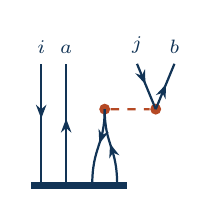
\begin{tikzpicture}[fcidiagram,scale=1.0]
    \draw[amp] (-0.40,0) -- (1.30,0);
    \node[vtx] (h0) at (0.90,1.35) {}; \node[vtx] (h1) at (1.80,1.35) {}; \draw[vint] (h0) -- (h1);
    \draw[hline] (0.68,0) .. controls (0.68,0.7) and (0.90,0.7) .. (h0.center);
    \draw[pline] (1.12,0) .. controls (1.12,0.7) and (0.90,0.7) .. (h0.center);
    \draw[pline] (h1.center) -- (2.13,2.15) node[dlab,above] {$b$};
    \draw[hline] (h1.center) -- (1.47,2.15) node[dlab,above] {$j$};
    \draw[hline] (-0.22,0) -- (-0.22,2.15) node[dlab,above] {$i$};
    \draw[pline] (0.22,0) -- (0.22,2.15) node[dlab,above] {$a$};
\end{tikzpicture}\\
{\footnotesize driving} & {\footnotesize Fock, particle} & {\footnotesize Fock, hole} & {\footnotesize pp ladder} & {\footnotesize hh ladder} & {\footnotesize ring}
\end{tabular}

\vspace{0.5em}
\begin{tabular}{@{}c@{\hspace{2em}}c@{\hspace{2em}}c@{\hspace{2em}}c@{}}
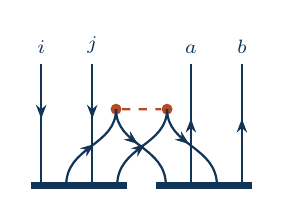
\begin{tikzpicture}[fcidiagram,scale=1.0]
    \draw[amp] (-0.40,0) -- (1.30,0);
    \draw[amp] (1.80,0) -- (3.50,0);
    \node[vtx] (h0) at (1.10,1.35) {}; \node[vtx] (h1) at (2.00,1.35) {}; \draw[vint] (h0) -- (h1);
    \draw[hline] (1.98,0) .. controls (1.98,0.7) and (1.10,0.7) .. (h0.center);
    \draw[pline] (0.22,0) .. controls (0.22,0.7) and (1.10,0.7) .. (h0.center);
    \draw[hline] (2.88,0) .. controls (2.88,0.7) and (2.00,0.7) .. (h1.center);
    \draw[pline] (1.12,0) .. controls (1.12,0.7) and (2.00,0.7) .. (h1.center);
    \draw[hline] (-0.22,0) -- (-0.22,2.15) node[dlab,above] {$i$};
    \draw[hline] (0.68,0) -- (0.68,2.15) node[dlab,above] {$j$};
    \draw[pline] (2.42,0) -- (2.42,2.15) node[dlab,above] {$a$};
    \draw[pline] (3.32,0) -- (3.32,2.15) node[dlab,above] {$b$};
\end{tikzpicture} & 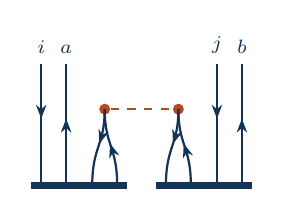
\begin{tikzpicture}[fcidiagram,scale=1.0]
    \draw[amp] (-0.40,0) -- (1.30,0);
    \draw[amp] (1.80,0) -- (3.50,0);
    \node[vtx] (h0) at (0.90,1.35) {}; \node[vtx] (h1) at (2.20,1.35) {}; \draw[vint] (h0) -- (h1);
    \draw[hline] (0.68,0) .. controls (0.68,0.7) and (0.90,0.7) .. (h0.center);
    \draw[pline] (1.12,0) .. controls (1.12,0.7) and (0.90,0.7) .. (h0.center);
    \draw[hline] (1.98,0) .. controls (1.98,0.7) and (2.20,0.7) .. (h1.center);
    \draw[pline] (2.42,0) .. controls (2.42,0.7) and (2.20,0.7) .. (h1.center);
    \draw[hline] (-0.22,0) -- (-0.22,2.15) node[dlab,above] {$i$};
    \draw[pline] (0.22,0) -- (0.22,2.15) node[dlab,above] {$a$};
    \draw[hline] (2.88,0) -- (2.88,2.15) node[dlab,above] {$j$};
    \draw[pline] (3.32,0) -- (3.32,2.15) node[dlab,above] {$b$};
\end{tikzpicture} & 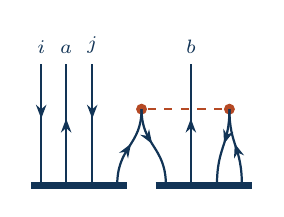
\begin{tikzpicture}[fcidiagram,scale=1.0]
    \draw[amp] (-0.40,0) -- (1.30,0);
    \draw[amp] (1.80,0) -- (3.50,0);
    \node[vtx] (h0) at (1.55,1.35) {}; \node[vtx] (h1) at (3.10,1.35) {}; \draw[vint] (h0) -- (h1);
    \draw[hline] (1.98,0) .. controls (1.98,0.7) and (1.55,0.7) .. (h0.center);
    \draw[pline] (1.12,0) .. controls (1.12,0.7) and (1.55,0.7) .. (h0.center);
    \draw[hline] (2.88,0) .. controls (2.88,0.7) and (3.10,0.7) .. (h1.center);
    \draw[pline] (3.32,0) .. controls (3.32,0.7) and (3.10,0.7) .. (h1.center);
    \draw[hline] (-0.22,0) -- (-0.22,2.15) node[dlab,above] {$i$};
    \draw[pline] (0.22,0) -- (0.22,2.15) node[dlab,above] {$a$};
    \draw[hline] (0.68,0) -- (0.68,2.15) node[dlab,above] {$j$};
    \draw[pline] (2.42,0) -- (2.42,2.15) node[dlab,above] {$b$};
\end{tikzpicture} & \begin{tikzpicture}[fcidiagram,scale=1.0]
    \draw[amp] (-0.40,0) -- (1.30,0);
    \draw[amp] (1.80,0) -- (3.50,0);
    \node[vtx] (h0) at (0.00,1.35) {}; \node[vtx] (h1) at (1.55,1.35) {}; \draw[vint] (h0) -- (h1);
    \draw[hline] (-0.22,0) .. controls (-0.22,0.7) and (0.00,0.7) .. (h0.center);
    \draw[pline] (0.22,0) .. controls (0.22,0.7) and (0.00,0.7) .. (h0.center);
    \draw[hline] (1.98,0) .. controls (1.98,0.7) and (1.55,0.7) .. (h1.center);
    \draw[pline] (1.12,0) .. controls (1.12,0.7) and (1.55,0.7) .. (h1.center);
    \draw[hline] (0.68,0) -- (0.68,2.15) node[dlab,above] {$j$};
    \draw[pline] (2.42,0) -- (2.42,2.15) node[dlab,above] {$b$};
    \draw[hline] (2.88,0) -- (2.88,2.15) node[dlab,above] {$i$};
    \draw[pline] (3.32,0) -- (3.32,2.15) node[dlab,above] {$a$};
\end{tikzpicture}\\
{\footnotesize $Q_a$} & {\footnotesize $Q_b$} & {\footnotesize $Q_c$} & {\footnotesize $Q_d$}
\end{tabular}
\end{center}
\begin{align*}
0={}&\as abij+P(ab)f_{bc}t_{ij}^{ac}-P(ij)f_{kj}t_{ik}^{ab}
 +\tfrac12\as abcd\,t_{ij}^{cd}+\tfrac12\as klij\,t_{kl}^{ab}+P(ij)P(ab)\as kbcj\,t_{ik}^{ac}\\
 &+\tfrac14\as klcd\,t_{ij}^{cd}t_{kl}^{ab}
 +\tfrac12P(ij)P(ab)\as klcd\,t_{ik}^{ac}t_{jl}^{bd}
 -\tfrac12P(ab)\as klcd\,t_{ij}^{ac}t_{kl}^{bd}
 -\tfrac12P(ij)\as klcd\,t_{ik}^{ab}t_{jl}^{cd}
\end{align*}
Ten diagrams, ten terms, in the same order. The same pictures are diagrams (1), (4)--(8) and (12)--(15) of the CCSD doubles equation in chapter 10, section 10.14; next week the other twenty-one, with $T_1$.
\end{frame}

\begin{frame}[shrink=4]{What iterating the equation sums}
\small
Write the equation as $D\,t=\as abij+L[t]+Q[t,t]$ ($L$: off-diagonal Fock, ladders, ring; $Q$: the four quadratic terms) and iterate from $t=0$:
\begin{center}
\renewcommand{\arraystretch}{1.35}
\begin{tabular}{lll}
\toprule
iteration & amplitude & the energy $\tfrac14\sum\as ijab t_{ij}^{ab}$ contains\\
\midrule
1 & $t^{[1]}=\as abij/D$ & second order (MP2)\\
2 & $t^{[2]}=(\as abij+L[t^{[1]}]+Q[t^{[1]},t^{[1]}])/D$ & $+$ third order: pp ladder, hh ladder, ring;\\
 & & $+$ the quadruples part of fourth order\\
3 & \dots & $+$ doubles part of fourth order, parts of fifth, \dots\\
$\infty$ & CCD & ladders, rings and their couplings to all orders\\
\bottomrule
\end{tabular}
\end{center}
\numbox{Pairing model, four levels, four particles, $g=0.5$ (Fock partition): $E^{(2)}=-0.062393$, $E^{(3)}=-0.016518$. Iteration 1: $-0.062393$. Iteration 2: $-0.078243=E^{(2)}+E^{(3)}+0.000669$, the last number from $Q[t^{[1]},t^{[1]}]$. Converged CCD: $-0.083362$. Exact: $-0.083226$.}
Each iteration puts a bar where a bare interaction (divided by $D$) stood: the diagrams of perturbation theory grow from the bottom.
\end{frame}

\begin{frame}[shrink=1]{Pause to think \#6}
\thinkq{3}{In a Hartree-Fock basis the fourth-order energy is usually split according to the intermediate states in the middle of the diagram: singles, doubles, triples and quadruples, $E^{(4)}=E^{(4)}_S+E^{(4)}_D+E^{(4)}_T+E^{(4)}_Q$.
\begin{enumerate}
\item Which of the four does CCD contain? Which diagrams of today generate them?
\item For the pairing model of the midterms, why is CCD nevertheless complete through fourth order?
\item What is the first order at which CCD and the exact pairing energy differ, and which cluster operator is responsible?
\end{enumerate}}
\end{frame}

\begin{frame}[shrink=1]{Answer to pause \#6}
\thinka{%
\begin{enumerate}
\item $E^{(4)}_D$: the linear diagrams iterated twice (doubles all the way). $E^{(4)}_Q$: the quadratic diagrams with first-order bars -- two doubles side by side form a quadruple, closed back to a double by $\as klcd$. Missing: $E^{(4)}_S$ and $E^{(4)}_T$, which need $T_1$ and $T_3$ (both start at second order).
\item Seniority. The pairing interaction moves complete pairs: no single and no triple excitation of the reference has unbroken pairs, so $E^{(4)}_S=E^{(4)}_T=0$. (Week 46: fourth-order coefficients of CCD and of exact Rayleigh-Schr\"odinger theory agree to ten digits.)
\item Fifth order. The connected quadruple $T_4$ starts at third order in the wave function and reaches the energy at fifth. For four particles in four levels it is the only cluster CCD lacks.
\end{enumerate}
In general: CCD is correct through third order, CCSD too; CCSD(T) and CCSDT through fourth.}
\end{frame}

\begin{frame}[shrink=3]{CCD intermediates and computational cost}
With $o$ occupied and $v$ virtual orbitals, a direct four-index inner sum for each amplitude suggests $O(o^4v^4)$ work. Factor the quadratic contractions using
\begin{align*}
 \chi_{kj}&=\tfrac12\as{k}{l}{c}{d}t_{jl}^{cd},&
 \chi_{cb}&=-\tfrac12\as{k}{l}{c}{d}t_{kl}^{bd},\\
 \chi_{klij}&=\tfrac12\as{k}{l}{c}{d}t_{ij}^{cd},&
 \chi_{bkcj}&=\tfrac12\as{k}{l}{c}{d}t_{lj}^{db}.
\end{align*}
The four quadratic terms are then
\[
 \tfrac12\chi_{klij}t_{kl}^{ab}
 +P(ij)P(ab)\chi_{bkcj}t_{ik}^{ac}
 +P(ab)\chi_{cb}t_{ij}^{ac}
 -P(ij)\chi_{kj}t_{ik}^{ab}.
\]
Each intermediate is formed once per iteration. The principal dense contractions scale as
\[
 O(o^2v^4)\quad\text{(pp ladder)},\qquad
 O(o^4v^2)\quad\text{(hh ladder)},\qquad O(o^3v^3)\quad\text{(rings)}.
\]
If $o$ and $v$ grow proportionally to basis size $n$, CCD costs $O(n^6)$ per iteration and stores $O(o^2v^2)$ doubles amplitudes. Full CC, with excitation rank growing with particle number, is not polynomial-cost.
\end{frame}

% ======================================================================
\section[Friday 4: CCD in code]{Friday, lecture 4: CCD for the pairing model, in code}
% ======================================================================

\begin{frame}[shrink=13]{The pairing model in spin orbitals}
\small
The model of both midterms: $L$ doubly degenerate levels, spacing $\xi=1$, $N$ particles,
\[
 H=\xi\sum_{p=1}^{L}\sum_{\sigma=\pm}(p-1)\,\cre{p\sigma}\ann{p\sigma}
 -\frac g2\sum_{pq}\cre{p+}\cre{p-}\ann{q-}\ann{q+}.
\]
What a coupled-cluster code needs is the Fock matrix and the antisymmetrised two-body elements.
\begin{block}{Matrix elements}
\[
 \as{p{+}}{p{-}}{q{+}}{q{-}}=-\frac g2\quad\text{(and the antisymmetric partners), all others zero.}
\]
\[
 f_{pq}=h_{pq}+\sum_{i}\as piqi:\qquad
 f_{i\sigma,i\sigma}=\varepsilon_i-\frac g2,\qquad f_{a\sigma,a\sigma}=\varepsilon_a,\qquad f_{p\ne q}=0 .
\]
\[
 \Eref=\sum_i h_{ii}+\frac12\sum_{ij}\as ijij=2\sum_{p\le N/2}\varepsilon_p-\frac g2\cdot\frac N2
 \qquad(=2-g\ \text{for}\ L=4,\ N=4).
\]
\end{block}
\begin{itemize}
\item The reference -- the $N/2$ lowest levels filled -- is already the Hartree-Fock determinant: $f$ is diagonal (week 39: ``Hartree-Fock does nothing for the pairing model'').
\item Everything beyond $\Eref$ is correlation energy.
\end{itemize}
\end{frame}

\begin{frame}[shrink=3]{What the pairing interaction does to the ten terms}
\small
The interaction annihilates a \emph{pair} $(q{+},q{-})$ and creates a pair $(p{+},p{-})$. It never breaks a pair: seniority is conserved.
\begin{center}
\renewcommand{\arraystretch}{1.25}
\begin{tabular}{lll}
\toprule
block & non-zero? & consequence\\
\midrule
$\as abij$ & yes: pair $i\to$ pair $a$ & driving term for pair amplitudes only\\
$\as abcd$ & yes: pair $c\to$ pair $a$ & pp ladder\\
$\as klij$ & yes: pair $i\to$ pair $k$ & hh ladder\\
$\as klcd$ & yes: pair $c\to$ pair $k$ & all four quadratic terms\\
$\as kbcj$ & \alert{no} & \alert{the ring term vanishes}\\
$f'$ (off-diagonal) & no & Fock terms $=$ denominators\\
\bottomrule
\end{tabular}
\end{center}
\begin{itemize}
\item $\as kbcj$ would need the two created orbitals $k$ (occupied) and $b$ (empty) to be the two members of one pair: impossible.
\item No single and no triple excitation has all pairs unbroken: $T_1=T_3=0$ on the ground-state branch. For this model CCSD $=$ CCD (the code confirms it), and the first missing cluster is $T_4$.
\item The only non-zero amplitudes are $t_{i+\,i-}^{a+\,a-}$: one number per occupied level $i$ and empty level $a$.
\end{itemize}
\end{frame}

\begin{frame}{Pause to think \#7}
\thinkq{3}{Four levels, four particles: $n_o=n_v=4$ spin orbitals.
\begin{enumerate}
\item The array \texttt{t[i,j,a,b]} has $4^4=256$ entries. How many are non-zero in the CCD solution of the pairing model, and how many of those are independent?
\item The first-order amplitude is $\as abij/D_{ij}^{ab}$. Write down the four independent first-order amplitudes for general $g$.
\item Use them to obtain the second-order energy. (You know the answer in the other partition: $-\tfrac{7}{24}g^2$.)
\end{enumerate}}
\end{frame}

\begin{frame}[shrink=1]{Answer to pause \#7}
\thinka{%
\begin{enumerate}
\item Four pairs of levels $(i,a)\in\{1,2\}\times\{3,4\}$, each appearing with $2\times2$ orderings of the spin labels: $16$ non-zero entries, $4$ independent numbers $t_i^a\equiv t_{i+\,i-}^{a+\,a-}$.
\item $D=2(f_{ii}-f_{aa})=2(\varepsilon_i-\varepsilon_a)-g$ and $\as abij=-g/2$:
\[
 t_1^3=\frac{g/2}{4+g},\qquad t_1^4=\frac{g/2}{6+g},\qquad t_2^3=\frac{g/2}{2+g},\qquad t_2^4=\frac{g/2}{4+g}.
\]
\item $\Delta E=\tfrac14\sum\as ijab t_{ij}^{ab}$: each pair appears four times, so $\Delta E=-\tfrac g2\sum_{ia}t_i^a$,
\[
 E^{(2)}_{\rm MP}=-\frac{g^2}{4}\Bigl(\frac1{2+g}+\frac2{4+g}+\frac1{6+g}\Bigr)
 \ \xrightarrow{\ g\ \text{small}\ }\ -\frac{7}{24}g^2 .
\]
The $+g$ in the denominators is the Hartree-Fock shift of the hole energies. The two partitions differ at third order; their sums to all orders agree.
\end{enumerate}}
\end{frame}

\begin{frame}[shrink=3]{The program: four small classes}
\small
\texttt{week47.ipynb}, plain \texttt{numpy}. The structure mirrors the derivation.
\begin{center}
\renewcommand{\arraystretch}{1.3}
\begin{tabular}{lp{0.68\textwidth}}
\toprule
class & responsibility\\
\midrule
\texttt{PairingModel} & the physics: $h$, $\as pqrs$, the Fock matrix, $\Eref$; the exact energy from the space of unbroken pairs (6 configurations for $L=4$, $N=4$)\\
\texttt{CCD} & the method, for \emph{any} $f$ and $\as pqrs$: the ten terms, the residual, the energy, a damped Jacobi solver\\
\texttt{DeterminantSpace} & the referee: $e^{-T}He^{T}$ by brute force on bit strings (week 38), no Wick, no diagrams\\
\texttt{PairCCD} & the same theory reduced by hand to pair amplitudes $t_i^a$\\
\bottomrule
\end{tabular}
\end{center}
\begin{itemize}
\item The solver knows nothing about pairing; the model knows nothing about coupled cluster. Swap either. (Chapter 10 runs the same kind of solver on the pairing plus particle-hole model.)
\item Amplitudes are stored as \texttt{t[i, j, a, b]}, integrals as \texttt{v[p, q, r, s]} $=\as pqrs$; the occupied spin orbitals come first.
\item Order of work: write the terms, \emph{test them against the referee}, only then solve.
\end{itemize}
\end{frame}

\begin{frame}[fragile,shrink=7]{The model}
\begin{lstlisting}[style=big]
class PairingModel:
    """The pairing Hamiltonian in a spin-orbital basis."""

    def __init__(self, levels=4, particles=4, g=1.0, xi=1.0):
        self.n, self.n_occ = 2 * levels, particles
        self.h = np.diag([xi * (p // 2) for p in range(self.n)]).astype(float)
        self.v = np.zeros((self.n,) * 4)              # <pq||rs>, antisymmetrised
        for p in range(levels):
            for q in range(levels):
                a, b, c, d = 2 * p, 2 * p + 1, 2 * q, 2 * q + 1
                self.v[a, b, c, d] += -0.5 * g        # <p+ p- || q+ q-> = -g/2
                self.v[b, a, c, d] -= -0.5 * g
                self.v[a, b, d, c] -= -0.5 * g
                self.v[b, a, d, c] += -0.5 * g

    @property
    def fock(self):                                   # f_pq = h_pq + sum_i <pi||qi>
        return self.h + sum(self.v[:, i, :, i] for i in range(self.n_occ))
\end{lstlisting}
\small Spin orbital $2(p-1)$ is $(p,+)$, $2(p-1)+1$ is $(p,-)$. For $g=1$: \texttt{diag(fock)} $=(-\tfrac12,-\tfrac12,\tfrac12,\tfrac12,2,2,3,3)$, \texttt{reference\_energy} $=1$ (the property $\sum_ih_{ii}+\tfrac12\sum_{ij}\as ijij$ is not shown).
\end{frame}

\begin{frame}[fragile,shrink=10]{The ten terms: one line each}
\begin{lstlisting}[style=big]
    def terms(self, t):                    # t[i, j, a, b];  w = <kl||cd>
        es, Pij, Pab, w = np.einsum, self.Pij, self.Pab, self.voovv
        return {
            "drive":  self.vvvoo.transpose(2, 3, 0, 1).copy(),
            "fock_p": Pab(es("bc,ijac->ijab", self.fvv, t)),
            "fock_h": -Pij(es("kj,ikab->ijab", self.foo, t)),
            "pp":     0.5 * es("abcd,ijcd->ijab", self.vvvvv, t),
            "hh":     0.5 * es("klij,klab->ijab", self.voooo, t),
            "ring":   Pij(Pab(es("kbcj,ikac->ijab", self.vovvo, t))),
            "Qa":     0.25 * es("klcd,ijcd,klab->ijab", w, t, t, optimize=True),
            "Qb":     0.5 * Pij(Pab(es("klcd,ikac,jlbd->ijab", w, t, t, optimize=True))),
            "Qc":     -0.5 * Pab(es("klcd,ijac,klbd->ijab", w, t, t, optimize=True)),
            "Qd":     -0.5 * Pij(es("klcd,ikab,jlcd->ijab", w, t, t, optimize=True)),
        }
    def residual(self, t, keep=None):      # <Phi_ij^ab| Hbar |Phi_0>
        terms = self.terms(t)
        return sum(terms[k] for k in (keep or self.names))
    def energy(self, t):                   # 1/4 sum <ij||ab> t_ij^ab
        return 0.25 * float(np.einsum("ijab,ijab->", self.voovv, t))
\end{lstlisting}
\small The index strings are the formulas: \texttt{"kbcj,ikac->ijab"} is $\as kbcj t_{ik}^{ac}$. \texttt{Pij(x) = x - x.transpose(1,0,2,3)}, \texttt{Pab} likewise. \texttt{keep} switches diagrams on and off.
\end{frame}

\begin{frame}[fragile,shrink=6]{The solver}
\begin{lstlisting}[style=big]
    def solve(self, mix=1.0, tol=1e-12, max_iter=2000, keep=None, project=True):
        t = self.vvvoo.transpose(2, 3, 0, 1) / self.D      # first order: <ab||ij>/D
        for it in range(1, max_iter + 1):
            R = self.residual(t, keep)
            if abs(R).max() < tol:                         # converged on the residual
                break
            t = t + mix * R / self.D                       # damped Jacobi step
            if project:
                t = 0.25 * self.Pij(self.Pab(t))           # keep t antisymmetric
        return t
\end{lstlisting}
\begin{itemize}
\item $R(t)$ is the sum of the ten terms, \emph{including} the diagonal Fock terms. Since $R=-D\,t+(\text{everything else})$, the step $t\leftarrow t+R/D$ is the same as $t\leftarrow(\as abij+L[t]+Q[t,t])/D$.
\item Start: the first-order amplitude. Stop: when the largest residual is below the tolerance. The energy is not used as a criterion.
\item \texttt{mix} $=\alpha$ damps the step, $t\leftarrow t+\alpha R/D$. \texttt{keep} selects a subset of the diagrams.
\item \texttt{project}: only the antisymmetric part of the array \texttt{t} means anything. More on this at the end of the lecture.
\end{itemize}
\end{frame}

\begin{frame}[fragile,shrink=1]{The referee: test before you trust}
\small
A random Hamiltonian (eight spin orbitals, four particles, non-diagonal Fock matrix), random antisymmetric amplitudes, and the matrices of $H$ and $T_2$ in the space of $\binom84=70$ determinants, built with the bit-string code of week 38:
\begin{lstlisting}[style=big]
space = DeterminantSpace(8, 4)
H, T  = space.hamiltonian(h, v), space.cluster_operator(t)
comm1 = H @ T - T @ H                        # [H, T]
comm2 = 0.5 * (comm1 @ T - T @ comm1)        # 1/2 [[H, T], T]
Hbar  = expm_nilpotent(-T) @ H @ expm_nilpotent(T)   # finite power series
\end{lstlisting}
Project each on the doubly excited determinants and compare, group by group:
\numbox{\small
\begin{tabular}{@{}lll@{}}
\texttt{drive} & against $\mel{\Phi_{ij}^{ab}}{H}{\ph}$ & largest difference $0$\\
\texttt{fock\_p + fock\_h + pp + hh + ring} & against $\mel{\Phi_{ij}^{ab}}{[H,T]}{\ph}$ & $9\times10^{-15}$\\
\texttt{Qa + Qb + Qc + Qd} & against $\mel{\Phi_{ij}^{ab}}{\tfrac12[[H,T],T]}{\ph}$ & $4\times10^{-15}$\\
the full residual & against $\mel{\Phi_{ij}^{ab}}{e^{-T}He^{T}}{\ph}$ & $7\times10^{-15}$\\
& $\mel{\Phi_{ij}^{ab}}{\tfrac1{3!}[[[H,T],T],T]}{\ph}$ & $0$
\end{tabular}}
The referee uses no Wick theorem and no diagrams. A wrong sign or a missing $\tfrac12$ in any term shows up here at once -- before any physics is attempted.
\end{frame}

\begin{frame}[fragile]{Running it}
\small
\begin{columns}[T]
\column{0.37\textwidth}
\begin{lstlisting}[style=mid]
model = PairingModel(4, 4, g=0.5)
cc = CCD(model.fock, model.v,
         model.n_occ)
t = cc.solve(verbose=True)
\end{lstlisting}
\begin{lstlisting}[style=mid,language={}]
 it     E_corr        max|R|
  1  -0.062393162   7.33e-02
  2  -0.078242708   1.84e-02
  3  -0.082124438   4.48e-03
  4  -0.083063834   1.08e-03
  5  -0.083290411   2.61e-04
  ...
 10  -0.083362277   2.11e-07
  ...
 19  -0.083362335   5.77e-13
\end{lstlisting}
The first line is MP2. The residual falls by a factor of about four per iteration.
\column{0.63\textwidth}
\begin{block}{Four levels, four particles, $\xi=1$}
\centering\scriptsize\setlength{\tabcolsep}{3.5pt}
\begin{tabular}{rrrrr}
\toprule
$g$ & MP2 & CCD & exact & CCD $-$ exact\\
\midrule
0.25 & 1.73320261 & 1.73045621 & 1.73045985 & $-3.6\times10^{-6}$\\
0.50 & 1.43760684 & 1.41663766 & 1.41677428 & $-1.4\times10^{-4}$\\
1.00 & 0.78095238 & 0.63044275 & 0.63554847 & $-5.1\times10^{-3}$\\
1.50 & 0.05974026 & $-0.38416526$ & $-0.34819051$ & $-3.6\times10^{-2}$\\
2.00 & $-0.70833333$ & $-1.60959440$ & $-1.48965216$ & $-1.2\times10^{-1}$\\
\bottomrule
\end{tabular}
\end{block}
\begin{itemize}
\item Total energies, $\Eref=2-g$ included. ``Exact'' is the diagonalisation of the first midterm.
\item Four parts in a million at $g=0.25$, where MP2 is off in the third decimal.
\item CCD lies \emph{below} the exact energy, increasingly so.
\end{itemize}
\end{columns}
\end{frame}

\begin{frame}[shrink=1]{What each diagram contributes}
\small
The ten terms of the equation for the amplitude $t_1^3$ (pair in level 1 to level 3) at the converged solution -- they add up to zero:
\begin{center}
\renewcommand{\arraystretch}{1.0}
\begin{tabular}{llrr}
\toprule
term & meaning here & $g=0.5$ & $g=1.0$\\
\midrule
driving & $-g/2$ & $-0.25000$ & $-0.50000$\\
Fock, particle & $(f_{aa}+f_{bb})\,t$ & $+0.29355$ & $+0.67024$\\
Fock, hole & $-(f_{ii}+f_{jj})\,t$ & $+0.03669$ & $+0.16756$\\
pp ladder & pair hops between empty levels & $-0.03025$ & $-0.13855$\\
hh ladder & pair hops between occupied levels & $-0.05311$ & $-0.23101$\\
ring & & $0$ & $0$\\
$Q_a$ & & $-0.00643$ & $-0.06401$\\
$Q_b$ & & $-0.00269$ & $-0.02808$\\
$Q_c$ & & $+0.00780$ & $+0.07742$\\
$Q_d$ & & $+0.00444$ & $+0.04643$\\
\midrule
amplitude $t_1^3$ & & $0.073388$ & $0.167560$\\
\bottomrule
\end{tabular}
\end{center}
The two Fock terms are $-D\,t$; the driving term and the ladders balance them. $Q_a,Q_b$ and $Q_c,Q_d$ come with opposite signs and largely cancel: the net quadratic term is small, positive, and \emph{reduces} the amplitude.
\end{frame}

\begin{frame}[shrink=6]{Switching the diagrams on, group by group}
\small
\texttt{cc.solve(keep=[...])} solves the equation with a subset of the terms.
\begin{center}
\renewcommand{\arraystretch}{1.2}
\begin{tabular}{rrrrrr}
\toprule
$g$ & MP2 & linear CCD & CID & CCD & exact\\
 & {\footnotesize driving only} & {\footnotesize + ladders} & {\footnotesize + ladders $-\Delta E\,C$} & {\footnotesize + ladders + $Q$} & \\
\midrule
0.25 & 1.73320261 & 1.73036649 & 1.73050700 & 1.73045621 & 1.73045985\\
0.50 & 1.43760684 & 1.41489362 & 1.41759645 & 1.41663766 & 1.41677428\\
1.00 & 0.78095238 & 0.59090909 & 0.64890655 & 0.63044275 & 0.63554847\\
1.50 & 0.05974026 & $-0.65384615$ & $-0.29113175$ & $-0.38416526$ & $-0.34819051$\\
2.00 & $-0.70833333$ & $-2.75000000$ & $-1.35208670$ & $-1.60959440$ & $-1.48965216$\\
\bottomrule
\end{tabular}
\end{center}
\begin{itemize}
\item \textbf{Linear CCD}: the ladders to all orders with nothing to stop them. It over-correlates at every coupling; the closed form $\Eref-g^2(7+2g)/(2(12-g^2))$ has a pole at $g=2\sqrt3$.
\item \textbf{CID} replaces the quadratic terms by the disconnected $-\Delta E\,C$ (Thursday): variational, hence above the exact energy -- and not size extensive.
\item \textbf{CCD}: the connected quadratic terms. Error at $g=1$: $0.045$ (linear), $0.013$ (CID), $0.005$ (CCD).
\item The missing piece is the connected quadruple $T_4$ -- three frames ahead.
\end{itemize}
\end{frame}

\begin{frame}[shrink=3]{Reduction to pair amplitudes: CCD in four unknowns}
\small
Write $T_2=\sum_{ia}t_i^a\,P_a^\dagger P_i$ with $P_p^\dagger=\cre{p+}\cre{p-}$; now $i,j$ label occupied \emph{levels}, $a,b$ empty levels, $G=g/2$ and $\varepsilon_p=\xi(p-1)$. Inserting the pairing matrix elements in the ten terms:
\begin{align*}
 0={}&\underbrace{-G}_{\text{driving}}
 +\underbrace{2(\varepsilon_a-\varepsilon_i)\,t_i^a}_{\text{Fock}+\text{diagonal ladders}}
 \underbrace{-G\sum_{b\ne a}t_i^b}_{\text{pp ladder}}
 \underbrace{-G\sum_{j\ne i}t_j^a}_{\text{hh ladder}}\\
 &+\underbrace{G\,t_i^a\Bigl(\sum_bt_i^b+\sum_jt_j^a-t_i^a\Bigr)-G\sum_{j\ne i}\sum_{b\ne a}t_i^b\,t_j^a}_{Q_a+Q_b+Q_c+Q_d},
 \qquad \Delta E=-G\sum_{ia}t_i^a .
\end{align*}
\begin{itemize}
\item The ladders move the pair to another empty level, or bring it from another occupied one. Their diagonal parts ($b=a$, $j=i$: $-2G\,t_i^a$) cancel the Hartree-Fock shift $+2G\,t_i^a$ of the Fock term.
\item Equivalent ``unlinked'' form of the last line: $+G\,S\,t_i^a-G\sum_{j\ne i,b\ne a}(t_i^at_j^b+t_i^bt_j^a)$ with $S=\sum t$. The first piece is $-\Delta E\,t_i^a$; the second is the coupling to the quadruple, whose coefficient in $e^{T_2}\ket{\ph}$ is $t_i^at_j^b+t_i^bt_j^a$ (pairs commute: a plus sign).
\item For $L=4$, $N=4$: four coupled quadratic equations for $t_1^3,t_1^4,t_2^3,t_2^4$. This is exercise 5 of week 46.
\end{itemize}
\end{frame}

\begin{frame}[fragile,shrink=7]{Pair CCD: the whole residual in ten lines}
\begin{lstlisting}[style=mid]
class PairCCD:
    def __init__(self, levels=4, particles=4, g=1.0, xi=1.0):
        self.G, no = 0.5 * g, particles // 2
        eps = xi * np.arange(levels)
        self.eo, self.ev = eps[:no], eps[no:]
        self.e_ref = 2 * self.eo.sum() - self.G * no
        self.D = 2 * (self.eo[:, None] - self.ev[None, :]) - 2 * self.G   # 2 (f_ii - f_aa)

    def residual(self, t):                       # t[i, a]: occupied level i, empty level a
        G = self.G
        row, col = t.sum(axis=1, keepdims=True), t.sum(axis=0, keepdims=True)
        gap = 2 * (self.ev[None, :] - self.eo[:, None])
        lin = -G + gap * t - G * (row - t) - G * (col - t)
        cross = row * col - t * row - t * col + t * t       # sum_{j!=i, b!=a} t_i^b t_j^a
        return lin + G * t * (row + col - t) - G * cross
\end{lstlisting}
\numbox{\small $g=0.5$: $t_1^3=0.073388$, $t_1^4=0.047621$, $t_2^3=0.139052$, $t_2^4=0.073388$; $\Eref-G\sum t=1.4166376647$, the spin-orbital result to all digits; the same four numbers sit in \texttt{t[i,j,a,b]}, and every other entry is zero.}
\end{frame}

\begin{frame}[shrink=13]{What CCD misses: compare with the exact wave function}
\small
In intermediate normalisation the exact state in the space of unbroken pairs is
\[
 \ket{\Psi}=\ket{\ph}+\sum_{ia}C_i^a\,P_a^\dagger P_i\ket{\ph}+C_4\,P_3^\dagger P_4^\dagger P_2P_1\ket{\ph}
 \qquad\text{(1 + 4 + 1 configurations).}
\]
CCD puts $C_i^a\to t_i^a$ and \emph{builds} the quadruple from the doubles: $C_4\to t_1^3t_2^4+t_1^4t_2^3$. The exact theory has $C_4=C_1^3C_2^4+C_1^4C_2^3+T_4$.
\begin{center}
\renewcommand{\arraystretch}{1.2}
\begin{tabular}{rrrrrr}
\toprule
$g$ & $\max|t_i^a-C_i^a|$ & $C_4$ exact & $t\,t+t\,t$ (CCD) & $C\,C+C\,C$ & $T_4$\\
\midrule
0.25 & $1.2\times10^{-5}$ & 0.002437 & 0.002624 & 0.002623 & $-0.00019$\\
0.50 & $2.3\times10^{-4}$ & 0.010296 & 0.012008 & 0.011968 & $-0.0017$\\
1.00 & $3.9\times10^{-3}$ & 0.043571 & 0.060331 & 0.058655 & $-0.015$\\
1.50 & $1.7\times10^{-2}$ & 0.095860 & 0.157908 & 0.145085 & $-0.049$\\
2.00 & $3.9\times10^{-2}$ & 0.156976 & 0.301975 & 0.257769 & $-0.101$\\
\bottomrule
\end{tabular}
\end{center}
\begin{itemize}
\item The product of doubles is the bulk of the quadruple at weak coupling -- the idea behind $e^{T}$ -- but it \emph{overshoots}: the connected $T_4$ is negative and grows with $g$.
\item Too large a quadruple feeds back on the doubles through the quadratic terms: too much correlation energy. That is the over-correlation in the tables.
\end{itemize}
\end{frame}

\begin{frame}{Pause to think \#8}
\thinkq{3}{At every coupling in the tables the CCD energy lies \emph{below} the exact ground-state energy of the same Hamiltonian in the same basis.
\begin{enumerate}
\item Is there a bug? Which theorem seems to be violated, and why is it not?
\item CID lies above the exact energy, CCD below. Which would you trust for five pairs? For fifty?
\item What would you have to compute to get an upper bound from the CCD wave function $e^{T_2}\ket{\ph}$?
\end{enumerate}}
\end{frame}

\begin{frame}{Answer to pause \#8}
\thinka{%
\begin{enumerate}
\item No bug. The variational principle bounds a \emph{Rayleigh quotient} $\langle\Psi|H|\Psi\rangle/\langle\Psi|\Psi\rangle$. The CCD energy is the projection $\mel{\ph}{He^{T_2}}{\ph}$, with $\bra{\ph}$ on the left instead of $\bra{\ph}e^{T_2^\dagger}$. It is not an expectation value in any state and obeys no bound.
\item CCD. The error of CID grows faster than the system: for $M$ non-interacting copies its correlation energy grows like $\sqrt M$ instead of $M$ (week 38). The error of CCD per pair stays put. A bound that deteriorates with size is worth less than an unbounded error that does not.
\item $\mel{\ph}{e^{T_2^\dagger}He^{T_2}}{\ph}/\mel{\ph}{e^{T_2^\dagger}e^{T_2}}{\ph}$: neither series terminates. That is variational coupled cluster; its unitary cousin $e^{T-T^\dagger}$ is what a quantum computer prepares (chapter 10, section 10.15, and FYS5419).
\end{enumerate}}
\end{frame}

\begin{frame}[shrink=4]{Convergence of the iteration, and two traps}
\small
\begin{columns}[T]
\column{0.45\textwidth}
Iterations to $\max|R|<10^{-12}$ for $t\leftarrow t+\alpha R/D$ ($L=4$, $N=4$):
\begin{center}
\footnotesize\renewcommand{\arraystretch}{1.1}
\begin{tabular}{rrrrr}
\toprule
$g$ & $\alpha=1$ & $0.7$ & $0.5$ & $0.3$\\
\midrule
$0.25$ & 14 & 27 & 44 & 81\\
$0.50$ & 19 & 35 & 54 & 98\\
$1.00$ & 27 & 45 & 69 & 123\\
$2.00$ & 32 & 53 & 79 & 141\\
$4.00$ & 83 & 44 & 68 & 122\\
$-0.50$ & 36 & 18 & 30 & 58\\
$-1.00$ & -- & 86 & 33 & 62\\
$-1.50$ & -- & -- & -- & 66\\
\bottomrule
\end{tabular}
\end{center}
(--: no convergence in 600 iterations.)
\column{0.55\textwidth}
\begin{itemize}
\item Mixing costs iterations where plain Jacobi works and rescues it where it does not. The converged energy does not depend on $\alpha$.
\item Repulsive pairing, $g<0$: the smallest denominator is $2(\varepsilon_2-\varepsilon_3)-g=-2-g$. At $g=-2$ it vanishes and the Jacobi step is undefined -- the equations are not.
\end{itemize}
\warnbox{\small Only the part of \texttt{t[i,j,a,b]} that is antisymmetric in $(i,j)$ and $(a,b)$ enters $T_2$. Rounding errors feed the rest, and the Jacobi map does not damp it. Ten levels, ten particles, $g=0.75$: with the projection $t\leftarrow\tfrac14P(ij)P(ab)\,t$ after each step, 40 iterations; without it, $\max|R|>10^6$ after 102.}
\end{columns}
\vspace{0.3em}
Judge convergence on the residual, not on the energy alone. Production codes replace the mixing by DIIS extrapolation.
\end{frame}

\begin{frame}[shrink=3]{A larger model space, and why intermediates matter}
\small
\begin{columns}[T]
\column{0.55\textwidth}
Ten levels, ten particles: $\binom{10}{5}=252$ pair configurations, $\binom{20}{10}=184\,756$ determinants, $25$ pair amplitudes.
\begin{center}
\footnotesize\renewcommand{\arraystretch}{1.15}
\begin{tabular}{rrrrr}
\toprule
$g$ & $\Eref$ & CCD & exact & \% of $E_{\rm corr}$\\
\midrule
0.25 & 19.3750 & 19.316138 & 19.316179 & 100.07\\
0.50 & 18.7500 & 18.466936 & 18.469552 & 100.93\\
0.75 & 18.1250 & 17.325660 & 17.365243 & 105.2\\
1.00 & 17.5000 & 15.573598 & 15.901417 & 120.5\\
\bottomrule
\end{tabular}
\end{center}
With five pairs CCD deteriorates faster with $g$ than with two: more connected quadruples (and hextuples) are missing, and the pairing correlations are becoming collective -- the regime of BCS theory (chapter 7), where a single reference determinant is a poor starting point.
\column{0.45\textwidth}
\begin{block}{Cost of a quadratic term}
$\tfrac14\as klcd t_{ij}^{cd}t_{kl}^{ab}$ as one eight-index sum: $n_o^4n_v^4$ operations. With the intermediate
\[
 \chi_{klij}=\tfrac12\as klcd t_{ij}^{cd},\qquad Q_a=\tfrac12\chi_{klij}t_{kl}^{ab}
\]
it is two sums of $n_o^4n_v^2$.
\end{block}
\numbox{\small $n_o=n_v=12$: $0.28$ s against $1.4$ ms, same numbers. (\texttt{optimize=True} lets \texttt{einsum} find the intermediate.)}
The dressed vertices of Thursday are not only a way to understand the quadratic terms; they are how the terms are computed.
\end{columns}
\end{frame}

\begin{frame}{The pairing model: energies and errors}
\begin{center}
\tikzset{every picture/.style={scale=1}}\begin{tikzpicture}[scale=1]
\begin{axis}[name=energy,width=6.4cm,height=4.7cm,xlabel={$g$},ylabel={Energy},xmin=0,xmax=2,grid=major,legend style={font=\scriptsize,at={(.03,.03)},anchor=south west},tick label style={font=\scriptsize},label style={font=\small}]
\addplot[gray,dashed] coordinates {(0.025,1.975) (0.05,1.95) (0.075,1.925) (0.1,1.9) (0.125,1.875) (0.15,1.85) (0.175,1.825) (0.2,1.8) (0.225,1.775) (0.25,1.75) (0.275,1.725) (0.3,1.7) (0.325,1.675) (0.35,1.65) (0.375,1.625) (0.4,1.6) (0.425,1.575) (0.45,1.55) (0.475,1.525) (0.5,1.5) (0.525,1.475) (0.55,1.45) (0.575,1.425) (0.6,1.4) (0.625,1.375) (0.65,1.35) (0.675,1.325) (0.7,1.3) (0.725,1.275) (0.75,1.25) (0.775,1.225) (0.8,1.2) (0.825,1.175) (0.85,1.15) (0.875,1.125) (0.9,1.1) (0.925,1.075) (0.95,1.05) (0.975,1.025) (1,1) (1.025,0.975) (1.05,0.95) (1.075,0.925) (1.1,0.9) (1.125,0.875) (1.15,0.85) (1.175,0.825) (1.2,0.8) (1.225,0.775) (1.25,0.75) (1.275,0.725) (1.3,0.7) (1.325,0.675) (1.35,0.65) (1.375,0.625) (1.4,0.6) (1.425,0.575) (1.45,0.55) (1.475,0.525) (1.5,0.5) (1.525,0.475) (1.55,0.45) (1.575,0.425) (1.6,0.4) (1.625,0.375) (1.65,0.35) (1.675,0.325) (1.7,0.3) (1.725,0.275) (1.75,0.25) (1.775,0.225) (1.8,0.2) (1.825,0.175) (1.85,0.15) (1.875,0.125) (1.9,0.1) (1.925,0.075) (1.95,0.05) (1.975,0.025) (2,0)};\addlegendentry{HF}
\addplot[blue] coordinates {(0.025,1.974819266) (0.05,1.949283174) (0.075,1.923400624) (0.1,1.897180176) (0.125,1.87063007) (0.15,1.843758243) (0.175,1.816572342) (0.2,1.789079737) (0.225,1.761287541) (0.25,1.733202614) (0.275,1.704831583) (0.3,1.676180846) (0.325,1.647256589) (0.35,1.618064791) (0.375,1.588611234) (0.4,1.558901515) (0.425,1.528941051) (0.45,1.498735088) (0.475,1.468288709) (0.5,1.437606838) (0.525,1.40669425) (0.55,1.375555577) (0.575,1.344195313) (0.6,1.312617817) (0.625,1.280827323) (0.65,1.248827943) (0.675,1.216623671) (0.7,1.184218388) (0.725,1.151615867) (0.75,1.118819777) (0.775,1.085833685) (0.8,1.052661064) (0.825,1.019305292) (0.85,0.9857696578) (0.875,0.9520573629) (0.9,0.9181715265) (0.925,0.8841151867) (0.95,0.8498913042) (0.975,0.8155027646) (1,0.780952381) (1.025,0.7462428966) (1.05,0.711376987) (1.075,0.6763572625) (1.1,0.6411862701) (1.125,0.6058664955) (1.15,0.5704003655) (1.175,0.5347902496) (1.2,0.4990384615) (1.225,0.4631472617) (1.25,0.4271188582) (1.275,0.3909554088) (1.3,0.3546590224) (1.325,0.3182317605) (1.35,0.2816756386) (1.375,0.2449926276) (1.4,0.2081846552) (1.425,0.1712536071) (1.45,0.134201328) (1.475,0.09702962329) (1.5,0.05974025974) (1.525,0.0223349668) (1.55,-0.01518456242) (1.575,-0.05281667008) (1.6,-0.09055973266) (1.625,-0.12841216) (1.65,-0.1663723945) (1.675,-0.20443891) (1.7,-0.242610211) (1.725,-0.2808848322) (1.75,-0.3192613371) (1.775,-0.3577383176) (1.8,-0.3963143934) (1.825,-0.4349882108) (1.85,-0.4737584425) (1.875,-0.5126237866) (1.9,-0.5515829661) (1.925,-0.5906347282) (1.95,-0.6297778438) (1.975,-0.6690111067) (2,-0.7083333333)};\addlegendentry{MP2}
\addplot[red,thick] coordinates {(0.025,1.974816404) (0.05,1.949260385) (0.075,1.923324063) (0.1,1.896999532) (0.125,1.870278863) (0.15,1.843154121) (0.175,1.815617377) (0.2,1.787660721) (0.225,1.759276277) (0.25,1.730456214) (0.275,1.701192765) (0.3,1.671478238) (0.325,1.641305034) (0.35,1.610665661) (0.375,1.579552748) (0.4,1.547959064) (0.425,1.51587753) (0.45,1.483301237) (0.475,1.450223458) (0.5,1.416637665) (0.525,1.38253754) (0.55,1.347916992) (0.575,1.312770169) (0.6,1.27709147) (0.625,1.240875556) (0.65,1.204117359) (0.675,1.166812099) (0.7,1.128955282) (0.725,1.09054272) (0.75,1.051570527) (0.775,1.012035133) (0.8,0.9719332842) (0.825,0.9312620494) (0.85,0.8900188215) (0.875,0.84820132) (0.9,0.8058075915) (0.925,0.7628360095) (0.95,0.7192852736) (0.975,0.6751544068) (1,0.6304427536) (1.025,0.5851499753) (1.05,0.5392760461) (1.075,0.4928212476) (1.1,0.4457861632) (1.125,0.3981716715) (1.15,0.3499789392) (1.175,0.3012094141) (1.2,0.2518648167) (1.225,0.201947132) (1.25,0.1514586013) (1.275,0.100401713) (1.3,0.04877919386) (1.325,-0.00340600062) (1.35,-0.05615069517) (1.375,-0.1094515043) (1.4,-0.1633048419) (1.425,-0.2177069303) (1.45,-0.2726538104) (1.475,-0.3281413504) (1.5,-0.3841652556) (1.525,-0.4407210775) (1.55,-0.4978042227) (1.575,-0.5554099624) (1.6,-0.6135334405) (1.625,-0.6721696832) (1.65,-0.7313136067) (1.675,-0.7909600258) (1.7,-0.8511036621) (1.725,-0.9117391518) (1.75,-0.9728610535) (1.775,-1.034463855) (1.8,-1.096541983) (1.825,-1.159089806) (1.85,-1.222101645) (1.875,-1.285571778) (1.9,-1.349494447) (1.925,-1.413863864) (1.95,-1.478674217) (1.975,-1.543919677) (2,-1.6095944)};\addlegendentry{CCD}
\addplot[black,densely dotted,thick] coordinates {(0.025,1.974816404) (0.05,1.949260386) (0.075,1.923324071) (0.1,1.896999565) (0.125,1.870278966) (0.15,1.843154382) (0.175,1.815617953) (0.2,1.787661867) (0.225,1.759278382) (0.25,1.730459846) (0.275,1.701198722) (0.3,1.671487607) (0.325,1.641319259) (0.35,1.610686618) (0.375,1.579582829) (0.4,1.548001271) (0.425,1.515935575) (0.45,1.483379651) (0.475,1.450327709) (0.5,1.416774284) (0.525,1.382714256) (0.55,1.348142868) (0.575,1.313055749) (0.6,1.277448929) (0.625,1.241318857) (0.65,1.204662412) (0.675,1.167476919) (0.7,1.129760156) (0.725,1.091510365) (0.75,1.052726253) (0.775,1.013407002) (0.8,0.973552265) (0.825,0.9331621672) (0.85,0.8922373022) (0.875,0.850778727) (0.9,0.8087879536) (0.925,0.7662669401) (0.95,0.7232180789) (0.975,0.6796441835) (1,0.6355484736) (1.025,0.590934559) (1.05,0.5458064221) (1.075,0.500168399) (1.1,0.4540251604) (1.125,0.4073816912) (1.15,0.3602432696) (1.175,0.3126154463) (1.2,0.2645040232) (1.225,0.2159150315) (1.25,0.1668547112) (1.275,0.1173294894) (1.3,0.06734596005) (1.325,0.01691086348) (1.35,-0.03396893308) (1.375,-0.08528645464) (1.4,-0.1370346367) (1.425,-0.1892063427) (1.45,-0.2417943811) (1.475,-0.2947915206) (1.5,-0.3481905058) (1.525,-0.4019840709) (1.55,-0.4561649532) (1.575,-0.510725905) (1.6,-0.5656597055) (1.625,-0.620959171) (1.65,-0.6766171649) (1.675,-0.7326266062) (1.7,-0.7889804783) (1.725,-0.8456718353) (1.75,-0.9026938096) (1.775,-0.960039617) (1.8,-1.017702562) (1.825,-1.075676044) (1.85,-1.133953559) (1.875,-1.192528703) (1.9,-1.251395177) (1.925,-1.310546788) (1.95,-1.369977453) (1.975,-1.429681197) (2,-1.489652155)};\addlegendentry{FCI}
\end{axis}
\begin{axis}[at={(energy.east)},anchor=west,xshift=1.5cm,width=6.4cm,height=4.7cm,xlabel={$g$},ylabel={$|E-E_{\rm FCI}|$},ymode=log,xmin=0,xmax=2,grid=major,legend style={font=\scriptsize,at={(.97,.03)},anchor=south east},tick label style={font=\scriptsize},label style={font=\small}]
\addplot[blue] coordinates {(0.025,2.861955856e-06) (0.05,2.27886195e-05) (0.075,7.655250605e-05) (0.1,0.0001806103899) (0.125,0.0003511044763) (0.15,0.0006038613368) (0.175,0.0009543887317) (0.2,0.001417870452) (0.225,0.002009159318) (0.25,0.002742768486) (0.275,0.003632861212) (0.3,0.004693239249) (0.325,0.005937330059) (0.35,0.007378173009) (0.375,0.009028404778) (0.4,0.01090024416) (0.425,0.0130054765) (0.45,0.01535543796) (0.475,0.01796099984) (0.5,0.02083255326) (0.525,0.02397999424) (0.55,0.0274127097) (0.575,0.0311395642) (0.6,0.03516888807) (0.625,0.03950846668) (0.65,0.0441655314) (0.675,0.04914675214) (0.7,0.05445823176) (0.725,0.06010550237) (0.75,0.06609352366) (0.775,0.07242668329) (0.8,0.07910879939) (0.825,0.08614312517) (0.85,0.09353235556) (0.875,0.101278636) (0.9,0.1093835729) (0.925,0.1178482466) (0.95,0.1266732253) (0.975,0.1358585811) (1,0.1454039074) (1.025,0.1553083375) (1.05,0.1655705649) (1.075,0.1761888635) (1.1,0.1871611096) (1.125,0.1984848044) (1.15,0.210157096) (1.175,0.2221748033) (1.2,0.2345344384) (1.225,0.2472322301) (1.25,0.2602641469) (1.275,0.2736259193) (1.3,0.2873130623) (1.325,0.301320897) (1.35,0.3156445717) (1.375,0.3302790823) (1.4,0.3452192919) (1.425,0.3604599498) (1.45,0.3759957091) (1.475,0.3918211439) (1.5,0.4079307655) (1.525,0.4243190377) (1.55,0.4409803908) (1.575,0.4579092349) (1.6,0.4750999728) (1.625,0.492547011) (1.65,0.5102447703) (1.675,0.5281876963) (1.7,0.5463702673) (1.725,0.5647870031) (1.75,0.5834324725) (1.775,0.6023012994) (1.8,0.6213881691) (1.825,0.6406878336) (1.85,0.6601951163) (1.875,0.679904916) (1.9,0.6998122106) (1.925,0.7199120602) (1.95,0.7401996094) (1.975,0.7606700899) (2,0.781318822)};\addlegendentry{MP2}
\addplot[red,thick] coordinates {(0.025,3.031774831e-11) (0.05,9.910838816e-10) (0.075,7.686158376e-09) (0.1,3.306869556e-08) (0.125,1.030020358e-07) (0.15,2.615101451e-07) (0.175,5.765141831e-07) (0.2,1.146044301e-06) (0.225,2.104907588e-06) (0.25,3.63178425e-06) (0.275,5.95671481e-06) (0.3,9.36893138e-06) (0.325,1.422497631e-05) (0.35,2.095704167e-05) (0.375,3.008145352e-05) (0.4,4.220721611e-05) (0.425,5.80445229e-05) (0.45,7.841313429e-05) (0.475,0.0001042505164) (0.5,0.0001366196309) (0.525,0.0001767162641) (0.55,0.0002258757828) (0.575,0.0002855792061) (0.6,0.0003574584879) (0.625,0.000443300909) (0.65,0.0005450524877) (0.675,0.0006648203286) (0.7,0.0008048738404) (0.725,0.0009676447691) (0.75,0.001155726008) (0.775,0.001371869159) (0.8,0.001618980852) (0.825,0.001900117808) (0.85,0.002218480717) (0.875,0.002577406926) (0.9,0.002980362052) (0.925,0.003430930544) (0.95,0.00393280533) (0.975,0.004489776613) (1,0.005105719947) (1.025,0.005784583697) (1.05,0.006530376013) (1.075,0.007347151431) (1.1,0.008238997236) (1.125,0.009210019702) (1.15,0.01026433033) (1.175,0.01140603219) (1.2,0.01263920651) (1.225,0.01396789955) (1.25,0.01539610993) (1.275,0.01692777639) (1.3,0.01856676619) (1.325,0.0203168641) (1.35,0.02218176208) (1.375,0.02416504967) (1.4,0.02627020517) (1.425,0.02850058758) (1.45,0.03085942934) (1.475,0.03334982986) (1.5,0.03597474988) (1.525,0.03873700658) (1.55,0.04163926954) (1.575,0.04468405735) (1.6,0.04787373505) (1.625,0.05121051224) (1.65,0.05469644184) (1.675,0.05833341955) (1.7,0.06212318382) (1.725,0.0660673165) (1.75,0.07016724391) (1.775,0.07442423847) (1.8,0.07883942072) (1.825,0.08341376181) (1.85,0.0881480863) (1.875,0.09304307534) (1.9,0.09809927009) (1.925,0.1033170755) (1.95,0.108696764) (1.975,0.1142384802) (2,0.1199422445)};\addlegendentry{CCD}
\end{axis}
\end{tikzpicture}
\end{center}
\small MP2 uses the fixed-Fock partition. CCD over-correlates here. In this seniority-zero, four-particle model the missing independent cluster is $T_4$; $e^{T_2}$ supplies only the disconnected $T_2^2/2$. Including $T_4$ makes this model exact on the ground-state branch. Curves were recomputed from the six pair determinants.
\end{frame}

% ======================================================================
\section{Summary}
% ======================================================================

\begin{frame}{Summary of week 47}
\begin{itemize}
\item CCD: $\ket{\Psi}=e^{T_2}\ket{\ph}$, energy $\Delta E=\tfrac14\sum\as ijab t_{ij}^{ab}$, and one quadratic equation per amplitude with ten terms: driving, two Fock, two ladders, ring, four quadratic.
\item \textbf{Analytically}: contract $H_N$ with $T_2$ until a two-body operator is left and project with the lemma. Weights are (prefactors) $\times$ (equal patterns); the diagonal Fock terms are the denominators; the quadratic terms are the linear ones with dressed vertices; the disconnected $\Delta E\,t$ cancels.
\item \textbf{Diagrammatically}: one $H_N$ fragment on top, bars below, level bookkeeping; sign $(-1)^{h+l}$, $\tfrac12$ per equivalent pair, $P$ for inequivalent external lines; no denominators, no lines between bars, no unattached bars.
\item \textbf{In code}: each term is one \texttt{einsum}; test against $e^{-T}He^{T}$ in determinant space before solving; iterate $t\leftarrow t+\alpha R/D$ on the residual; antisymmetrise.
\item \textbf{Pairing model}: no ring term, no singles; four pair amplitudes for $L=4$, $N=4$; CCD is exact for one pair, $4\times10^{-6}$ off at $g=0.25$, below the exact energy and $0.12$ off at $g=2$. What is missing is $T_4$.
\end{itemize}
\end{frame}

\begin{frame}{Next week: the last week of the semester}
  \begin{exampleblock}{Week 48, Thursday November 26: coupled cluster with singles and doubles}
    \small
    $T=T_1+T_2$. What $e^{T_1}$ does (an orbital rotation: Thouless' theorem once more) and the CCSD equations obtained analytically from the CCD equations with a $T_1$-dressed Hamiltonian; the same equations diagrammatically -- three energy diagrams, fourteen for the singles, thirty-one for the doubles; intermediates; when singles matter; a look beyond CCSD.
  \end{exampleblock}
  \begin{exampleblock}{Week 48, Friday November 27: summary of the course, and the final oral exam}
    \small
    What we have done this semester, method by method, with the pairing model as the common thread; how the methods relate; the format and the syllabus of the final oral exam.
  \end{exampleblock}
  \vspace{0.4em}
  \small
  Reading: chapter 10, sections 10.7 (CCSD), 10.10 (when singles matter), 10.13 (beyond CCSD) and 10.14 (the diagrammatic derivation); Shavitt and Bartlett, chapters 9--10.\\[0.3em]
  No exercises this week or next. \textbf{Second midterm: deadline Monday November 23 at midnight.}
\end{frame}

% ======================================================================
\section{Answers to the week-46 exercises}
% ======================================================================

\begin{frame}[shrink=3]{Week-46 exercises 1 and 2: unlinked diagrams and factorisation}
\small
The full derivations are on the week-46 slides and in chapter 9, section 9.15; here the results.
\begin{block}{1. Linked and unlinked at third order}
The unlinked drawings in $\mel{\Phi_m}{RVRVRV}{\ph}$ fall in three families (answer to pause \#1, week 46): one closed one-vertex piece $E^{(1)}$ in either of two positions, cancelled by $-E^{(1)}[RVR^2V+R^2VRV]$; two such pieces, counted $+1-2$ and restored by $+(E^{(1)})^2R^3V$; one closed two-vertex piece in two time orderings, which sum by
$\frac1{D_m(D_m+D_n)D_m}+\frac1{D_n(D_m+D_n)D_m}=\frac1{D_m^2D_n}$ to $E^{(2)}V_{m0}/D_m^2$ and are cancelled by $-E^{(2)}R^2V$. Closing with a top vertex gives the principal term of $E^{(4)}$ and its three renormalisation terms $-E^{(1)}\langle\cdots\rangle$ (twice), $+(E^{(1)})^2\langle VR^3V\rangle$, $-E^{(2)}\langle VR^2V\rangle$.
\end{block}
\begin{block}{2. The factorisation theorem}
Induction on the last vertex: $S_{rs}=(S_{r-1,s}+S_{r,s-1})/(A_r+B_s)$ with the hypothesis for both terms gives $\frac{A_r+B_s}{A_r+B_s}\prod A_u^{-1}\prod B_v^{-1}$. With a closed component ($B_s=0$, boundary condition $S_{0s}=0$ from $Q$) the same recursion gives $\prod_{u<r}A_u^{-1}\prod_{v<s}B_v^{-1}\sum_{j<r}A_j^{-1}$. For $r=3$, $s=2$ (open deficits $a,b$; closed $c,0$) the five interleavings $A_1A_2B_1B_2$, $A_1B_1A_2B_2$, $A_1B_1B_2A_2$, $B_1A_1A_2B_2$, $B_1A_1B_2A_2$ sum to $\frac1{abc}\bigl(\frac1a+\frac1b\bigr)$: $E^{(2)}$ times an $R_0^2$ on either interval, i.e.\ the fifth-order folded terms $-E^{(2)}\langle WR_0^2WR_0W\rangle-E^{(2)}\langle WR_0WR_0^2W\rangle$.
\end{block}
\end{frame}

\begin{frame}[shrink=13]{Week-46 exercises 3, 4 and 5}
\small
\begin{block}{3. Exclusion-principle-violating diagrams}
Two-level model: four complete contractions, all with $h=2$. Same matching of particles and holes at both pairs of vertices: two pairings, $l=2$, $+2F$, unlinked. Opposite matchings: two pairings, $l=1$, $-2F$, linked; $F=|g|^4/(2D^3)$. The folded term removes $+2F$ and $E^{(4)}=-2F=+|g|^4/\Delta^3$, all of it from diagrams that violate the exclusion principle.

One pair in two levels of the pairing model: the same structure with $g\to-g/2$ and $\Delta=2\xi$. Two simultaneous pair excitations would need two pairs in level 1 -- an EPV intermediate state -- and
$E-\Eref=\tfrac12\bigl(\Delta-\sqrt{\Delta^2+g^2}\bigr)=-\frac{g^2}{4\Delta}+\frac{g^4}{16\Delta^3}-\cdots$: the fourth-order term again comes entirely from linked EPV diagrams. Nothing changes.
\end{block}
\begin{block}{4. The exponential ansatz}
Thursday, lecture 1 of this week (commuting excitations, $C_n$ in terms of $T$'s, factorisation, termination) and the corresponding frames of week 46.
\end{block}
\begin{block}{5. CCD for the pairing model}
Friday, lecture 4: the ring term and $T_1$ vanish by seniority; the pair-amplitude equation and its ten-line residual; $g=0.5$: $t=(0.073388,\,0.047621,\,0.139052,\,0.073388)$ and $E=1.41663766$, as in the table. \texttt{week47.ipynb}, sections 5--6.
\end{block}
\end{frame}

\begin{frame}{References}
\small
\begin{itemize}
\item Lecture notes, chapter 10: sections 10.1--10.6, 10.9 and 10.14. Programs \texttt{BookPrograms/chapter10/coupledcluster.py} (general CCSD/CCD solver with intermediates) and \texttt{ccsd\_diagrams.py} (the diagrams, checked against $e^{-T}He^{T}$).
\item I. Shavitt and R. J. Bartlett, \emph{Many-Body Methods in Chemistry and Physics} (Cambridge, 2009), chapters 9 and 10.
\item T. D. Crawford and H. F. Schaefer, ``An introduction to coupled cluster theory for computational chemists'', \emph{Rev. Comput. Chem.} \textbf{14}, 33 (2000).
\item R. J. Bartlett and M. Musia\l{}, ``Coupled-cluster theory in quantum chemistry'', \emph{Rev. Mod. Phys.} \textbf{79}, 291 (2007), \href{https://doi.org/10.1103/RevModPhys.79.291}{doi:10.1103/RevModPhys.79.291}.
\item J. \v{C}\'i\v{z}ek, ``On the correlation problem in atomic and molecular systems'', \emph{J. Chem. Phys.} \textbf{45}, 4256 (1966) -- the CCD equations, derived with diagrams.
\item G. Hagen, T. Papenbrock, M. Hjorth-Jensen and D. J. Dean, ``Coupled-cluster computations of atomic nuclei'', \emph{Rep. Prog. Phys.} \textbf{77}, 096302 (2014).
\item T. Papenbrock, \href{https://nucleartalent.github.io/ManyBody2018/doc/pub/CCM/html/CCM.html}{The Coupled-Cluster Method}, Nuclear TALENT course notes (2018): the pairing-model CCD program \texttt{CCD\_PairingModel.py}.
\end{itemize}
\end{frame}

\end{document}
